\documentclass{beamer}
\setbeamertemplate{navigation symbols}{}
\usepackage{comment}

\setbeamercolor{frametitle}{fg=black,bg=white}
\setbeamercolor{title}{fg=black,bg=yellow!85!orange}
\usetheme{AnnArbor}

\usepackage{textpos} % package for the positioning
\usepackage{listings}
\usepackage{xcolor}
\usepackage[most]{tcolorbox}
\usepackage{mathtools}
\usepackage{graphicx}
\usepackage{graphbox}
\usepackage{movie15}
\usepackage{caption}
\DeclareCaptionType{code}[Code Listing][List of Code Listings] 

\definecolor{codegreen}{rgb}{0,0.6,0}
\definecolor{codegray}{rgb}{0.5,0.5,0.5}
\definecolor{codepurple}{rgb}{0.58,0,0.82}
\definecolor{backcolour}{rgb}{0.95,0.95,0.92} 
\lstdefinestyle{mystyle}{
    backgroundcolor=\color{backcolour},   
    commentstyle=\color{codegreen},
    keywordstyle=\color{magenta},
    numberstyle=\tiny\color{codegray},
    stringstyle=\color{codepurple},
    basicstyle=\ttfamily\footnotesize,
    breakatwhitespace=false,         
    breaklines=true,                 
    captionpos=b,                    
    keepspaces=true,                 
    numbers=left,                    
    numbersep=5pt,                  
    showspaces=false,                
    showstringspaces=false,
    showtabs=false,                  
    tabsize=2
}

\lstset{style=mystyle}

\lstdefinelanguage
   [x64]{Assembler}     % add a "x64" dialect of Assembler
   [x86masm]{Assembler} % based on the "x86masm" dialect
   % with these extra keywords:
   {morekeywords={CDQE,CQO,CMPSQ,CMPXCHG16B,JRCXZ,LODSQ,MOVSXD, %
                  POPFQ,PUSHFQ,SCASQ,STOSQ,IRETQ,RDTSCP,SWAPGS, %
                  rax,rdx,rcx,rbx,rsi,rdi,rsp,rbp, %
                  r8,r8d,r8w,r8b,r9,r9d,r9w,r9b, %
                  r10,r10d,r10w,r10b,r11,r11d,r11w,r11b, %
                  r12,r12d,r12w,r12b,r13,r13d,r13w,r13b, %
                  r14,r14d,r14w,r14b,r15,r15d,r15w,r15b}} %


\beamersetuncovermixins{\opaqueness<1>{25}}{\opaqueness<2->{15}}

%Copyright
\addtobeamertemplate{frametitle}{}{%
\begin{textblock*}{50mm}(0cm,-1.25cm)
\color{yellow!85!orange}
\tiny{Copyright \copyright 2024 CNM.}
\end{textblock*}}

% position the logo
\addtobeamertemplate{frametitle}{}{%
\begin{textblock*}{100mm}(11.4cm,-1.3cm)

\includegraphics[height=1cm,width=1cm,keepaspectratio]{fig/ddclogotransparent.png}
\end{textblock*}}

\AtBeginSection[]{
  \begin{frame}
  \vfill
  \centering
  \begin{beamercolorbox}[sep=8pt,center,shadow=true,rounded=true]{title}
    \usebeamerfont{title}\insertsectionhead\par%
  \end{beamercolorbox}
  \vfill
  \end{frame}
}

\begin{document}
\title{Quantum Technician Bootcamp}
\author{Brian Rashap}
\date{September 2025} 

\begin{frame}
\titlepage
\end{frame}

\section{Introduction}

\begin{frame}\frametitle{Instructional team}
A physicist, an engineer, and a technician walk into a classroom...
\end{frame}

\begin{frame}
\frametitle{The Engineer: Brian Rashap, Ph.D.}
\begin{columns}
\begin{column}{6.5cm}
\begin{itemize}
\item Proud husband of Krista and father of Shelby (27) and Ethan (23)
\item Electrical Engineer (Michigan) with 23 years industrial experience (Intel)
\item Created and taught IoT Bootcamp for 5 years (and going)
\item Hobbies: painting, cycling, swimming, reading, spending time with family
\end{itemize}
\end{column}
\begin{column}{4.5cm}
\begin{center}
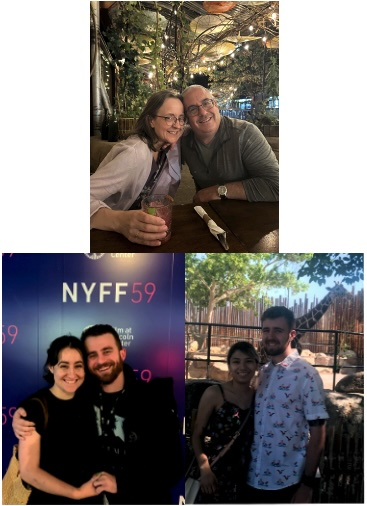
\includegraphics[width=4.5cm]{fig/rashapfamily.jpg}
\end{center}
\end{column}
\end{columns}
\end{frame}

\begin{frame}
\frametitle{The Physicist: Megan Ivory}
\begin{columns}
\begin{column}{8cm}
\begin{itemize}
\item Foster mom to two cats, Joey and Tessa; auntie to two humans, Liana and Azeria
\item PhD in atomic physics (William and Mary), startup ColdQuanta (now Infleqtion), Univ of Washington, Sandia since 2019 working on atomic clocks, quantum computers, and quantum programs like QuLL!
\item Outside hobbies: trail running, hiking, gardening, backpacking, trad climbing, canyoneering, and skiing
\item Inside hobbies: cooperative board games, reading trashy fantasy series, acting/writing
\end{itemize}
\end{column}
\begin{column}{3.5cm}
\begin{center}
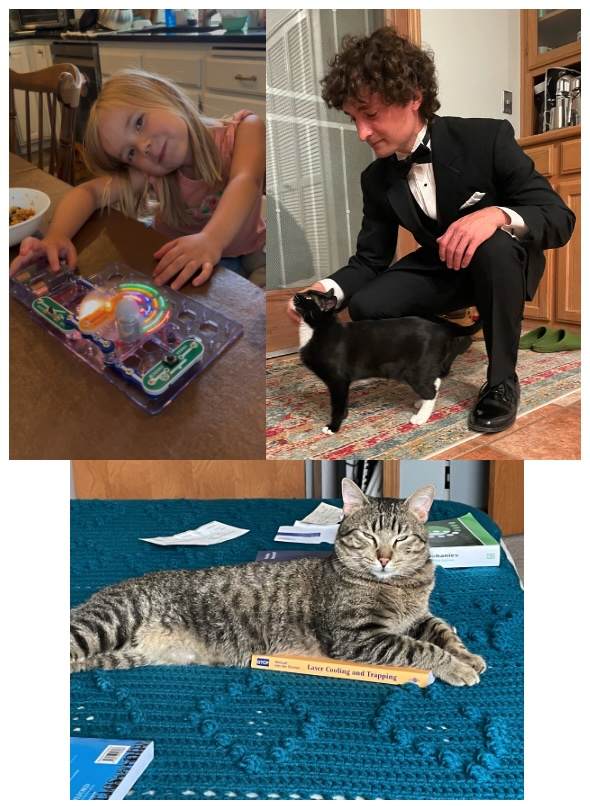
\includegraphics[width=3.5cm]{fig/meganfam.jpg}
\end{center}
\end{column}
\end{columns}

\vspace{0.5cm}

I’ve never taken a quantum information science class…
\end{frame}

\begin{frame}
\frametitle{The Technician: Shawn Morales}
\begin{columns}
\begin{column}{6cm}
\begin{itemize}
\item Blessed husband of Joy and proud father of Katelyn (29) and Kimber (28)
\item Intel Manufacturing Technician of 32 years
\item Worked on 26 different tools within Intel
\item Adore my time with family, mountain biking, and the great outdoors
\end{itemize}
\end{column}
\begin{column}{5cm}
\begin{center}
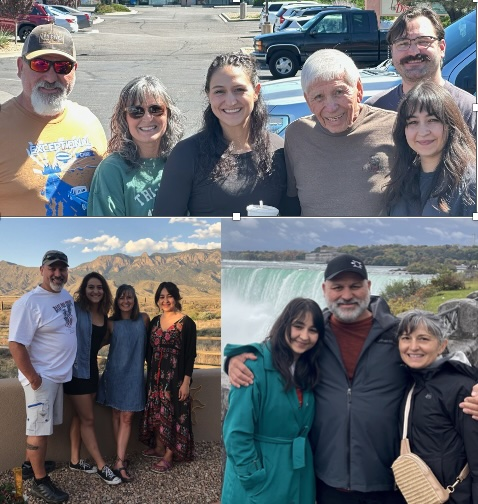
\includegraphics[width=4.5cm]{fig/shawn.jpg}
\end{center}
\end{column}
\end{columns}
\end{frame}

\begin{frame}\frametitle{Student Introductions}
\begin{itemize}
\item Your name
\item What were you up to before starting the bootcamp
\item Any prior experience with math, science, machining, etc.
\item What do you hope to get out of the bootcamp
\end{itemize}
\end{frame}

\begin{frame}\frametitle{Drinks, Lunch and Snacks}
\begin{itemize}
\item There is a kitchenette down the hall with coffee/tea, snacks, frig, microwave
\begin{itemize}
\item The rest of the room is the TSL Lab - please don't disturb it
\item Please clean up the area every time you use it.
\item Don't leave leftovers overnight in the frig
\end{itemize}
\item Drink are allowed in the QuLL, but not near the optical tables or vacuum systems
\item You can eat lunch in the QuLL, 
\begin{itemize}
\item There will be a mid-day 1 hour lunch break
\item Again, no food/drink near optical tables or vacuum systems
\item Tables wiped down at the end of lunch
\end{itemize}
\item No food trash in QuLL garbage can (use the kitchenette trash)
\end{itemize}
\end{frame}


\begin{frame}\frametitle{Class Rules}
\begin{itemize}
\item Respect each other. Help each other.
\item Ask questions. 
\item Be on time (let us know via Slack if you won't be here) 
\item Keep your workspace and the classroom neat and tidy.
\item If you are struggling, let us know. We are here to HELP!
\item Class hours
\begin{itemize}
\item Mon-Th: 8am to 5pm \footnote{Doors open at 7:50, please be in your seats ready to learn by 8:00} and Friday: 8am to 3pm \footnote{Occasionally on Friday there will be optional activities from 3 to 5}
\item Lunch Break: 1 hour near noon. Maybe combined with work time. 
\item Please respect the instructors' lunch break as well.
\end{itemize}
\item Phone Policy: phones should not be out or used during class
\begin{itemize}
\item No gaming, no surfing social media
\item If you need to take/make a call, please set out of the classroom
\item Exceptions: two-factor authentication, pictures of projects, class videos
\end{itemize}
\end{itemize}
\end{frame}

\begin{frame}\frametitle{Credit for Prior Learning (CPL)}
If students enroll in an academic program at CNM, they are eligible for up to 24 credits though CPL:

\begin{itemize}
\item Current CPL (will be finalized before December)
\begin{itemize}
\item MATH 1220 College Algebra
\item BCIS 1110 Fundamentals of Information Literacy and Systems
\item BUSA Business Professionalism
\end{itemize}
\item CPL that can be claimed starting in Fall 2026
\begin{itemize}
\item ENGT 10xx Optics
\item ENGT 20xx Laser and Photonics
\item CSCI 10xx Survey of Quantum Computing
\item CSCI 20xx Quantum Hardware
\end{itemize}




\end{itemize}


\end{frame}


\begin{frame}\frametitle{Foundation of lean Certificate}
\begin{center}

\includegraphics[width=8cm]{fig/nmmep.png} 
\end{center}
\end{frame}


\begin{frame}\frametitle{IPC Solder Certification}
\begin{columns}
\begin{column}{5.5cm}
	\begin{center}	
	
\includegraphics[width=5cm]{fig/ipc1.png} 
	\end{center}
\end{column}
\begin{column}{5.5cm}
	\begin{center}	
	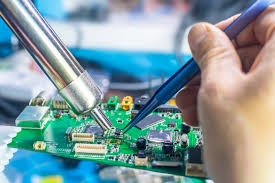
\includegraphics[width=5cm]{fig/ipc2.jpg} 
	\end{center}
\end{column}
\end{columns}
\end{frame}



\begin{frame}\frametitle{Important Attribute in an Employee}
\begin{columns}
\begin{column}{5cm}
\begin{itemize}
\item Tolerance of Ambiguity
\item Attention to Detail
\item Reliability 
\item Curiosity
\item Structured Problem Solving
\end{itemize}
\end{column}
\begin{column}{5cm}
\begin{center}
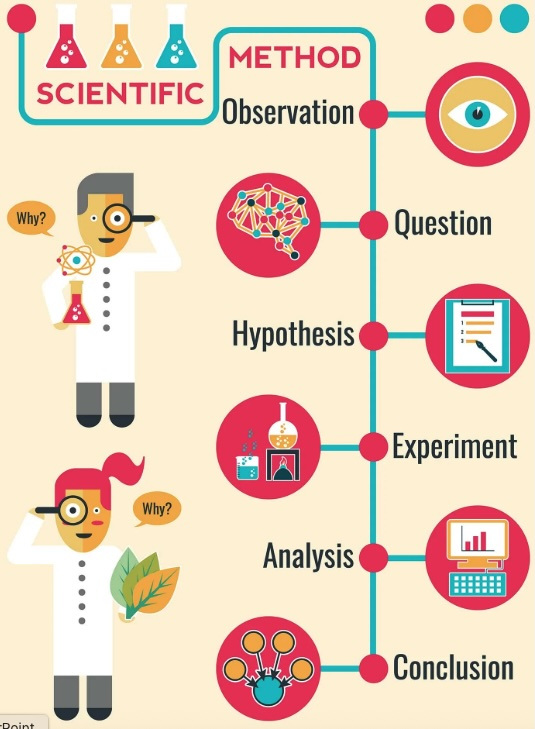
\includegraphics[width=3.5cm]{fig/scimeth.jpg}
\end{center}

\end{column}
\end{columns}


\vspace{1cm}

Note: employers regularly ask the instructional team for references, it is these attributes that we will be the basis of our recommendation. 
\end{frame}

\section{Overview: QIS in NM}

\begin{frame}\frametitle{Introduction}
\begin{center}
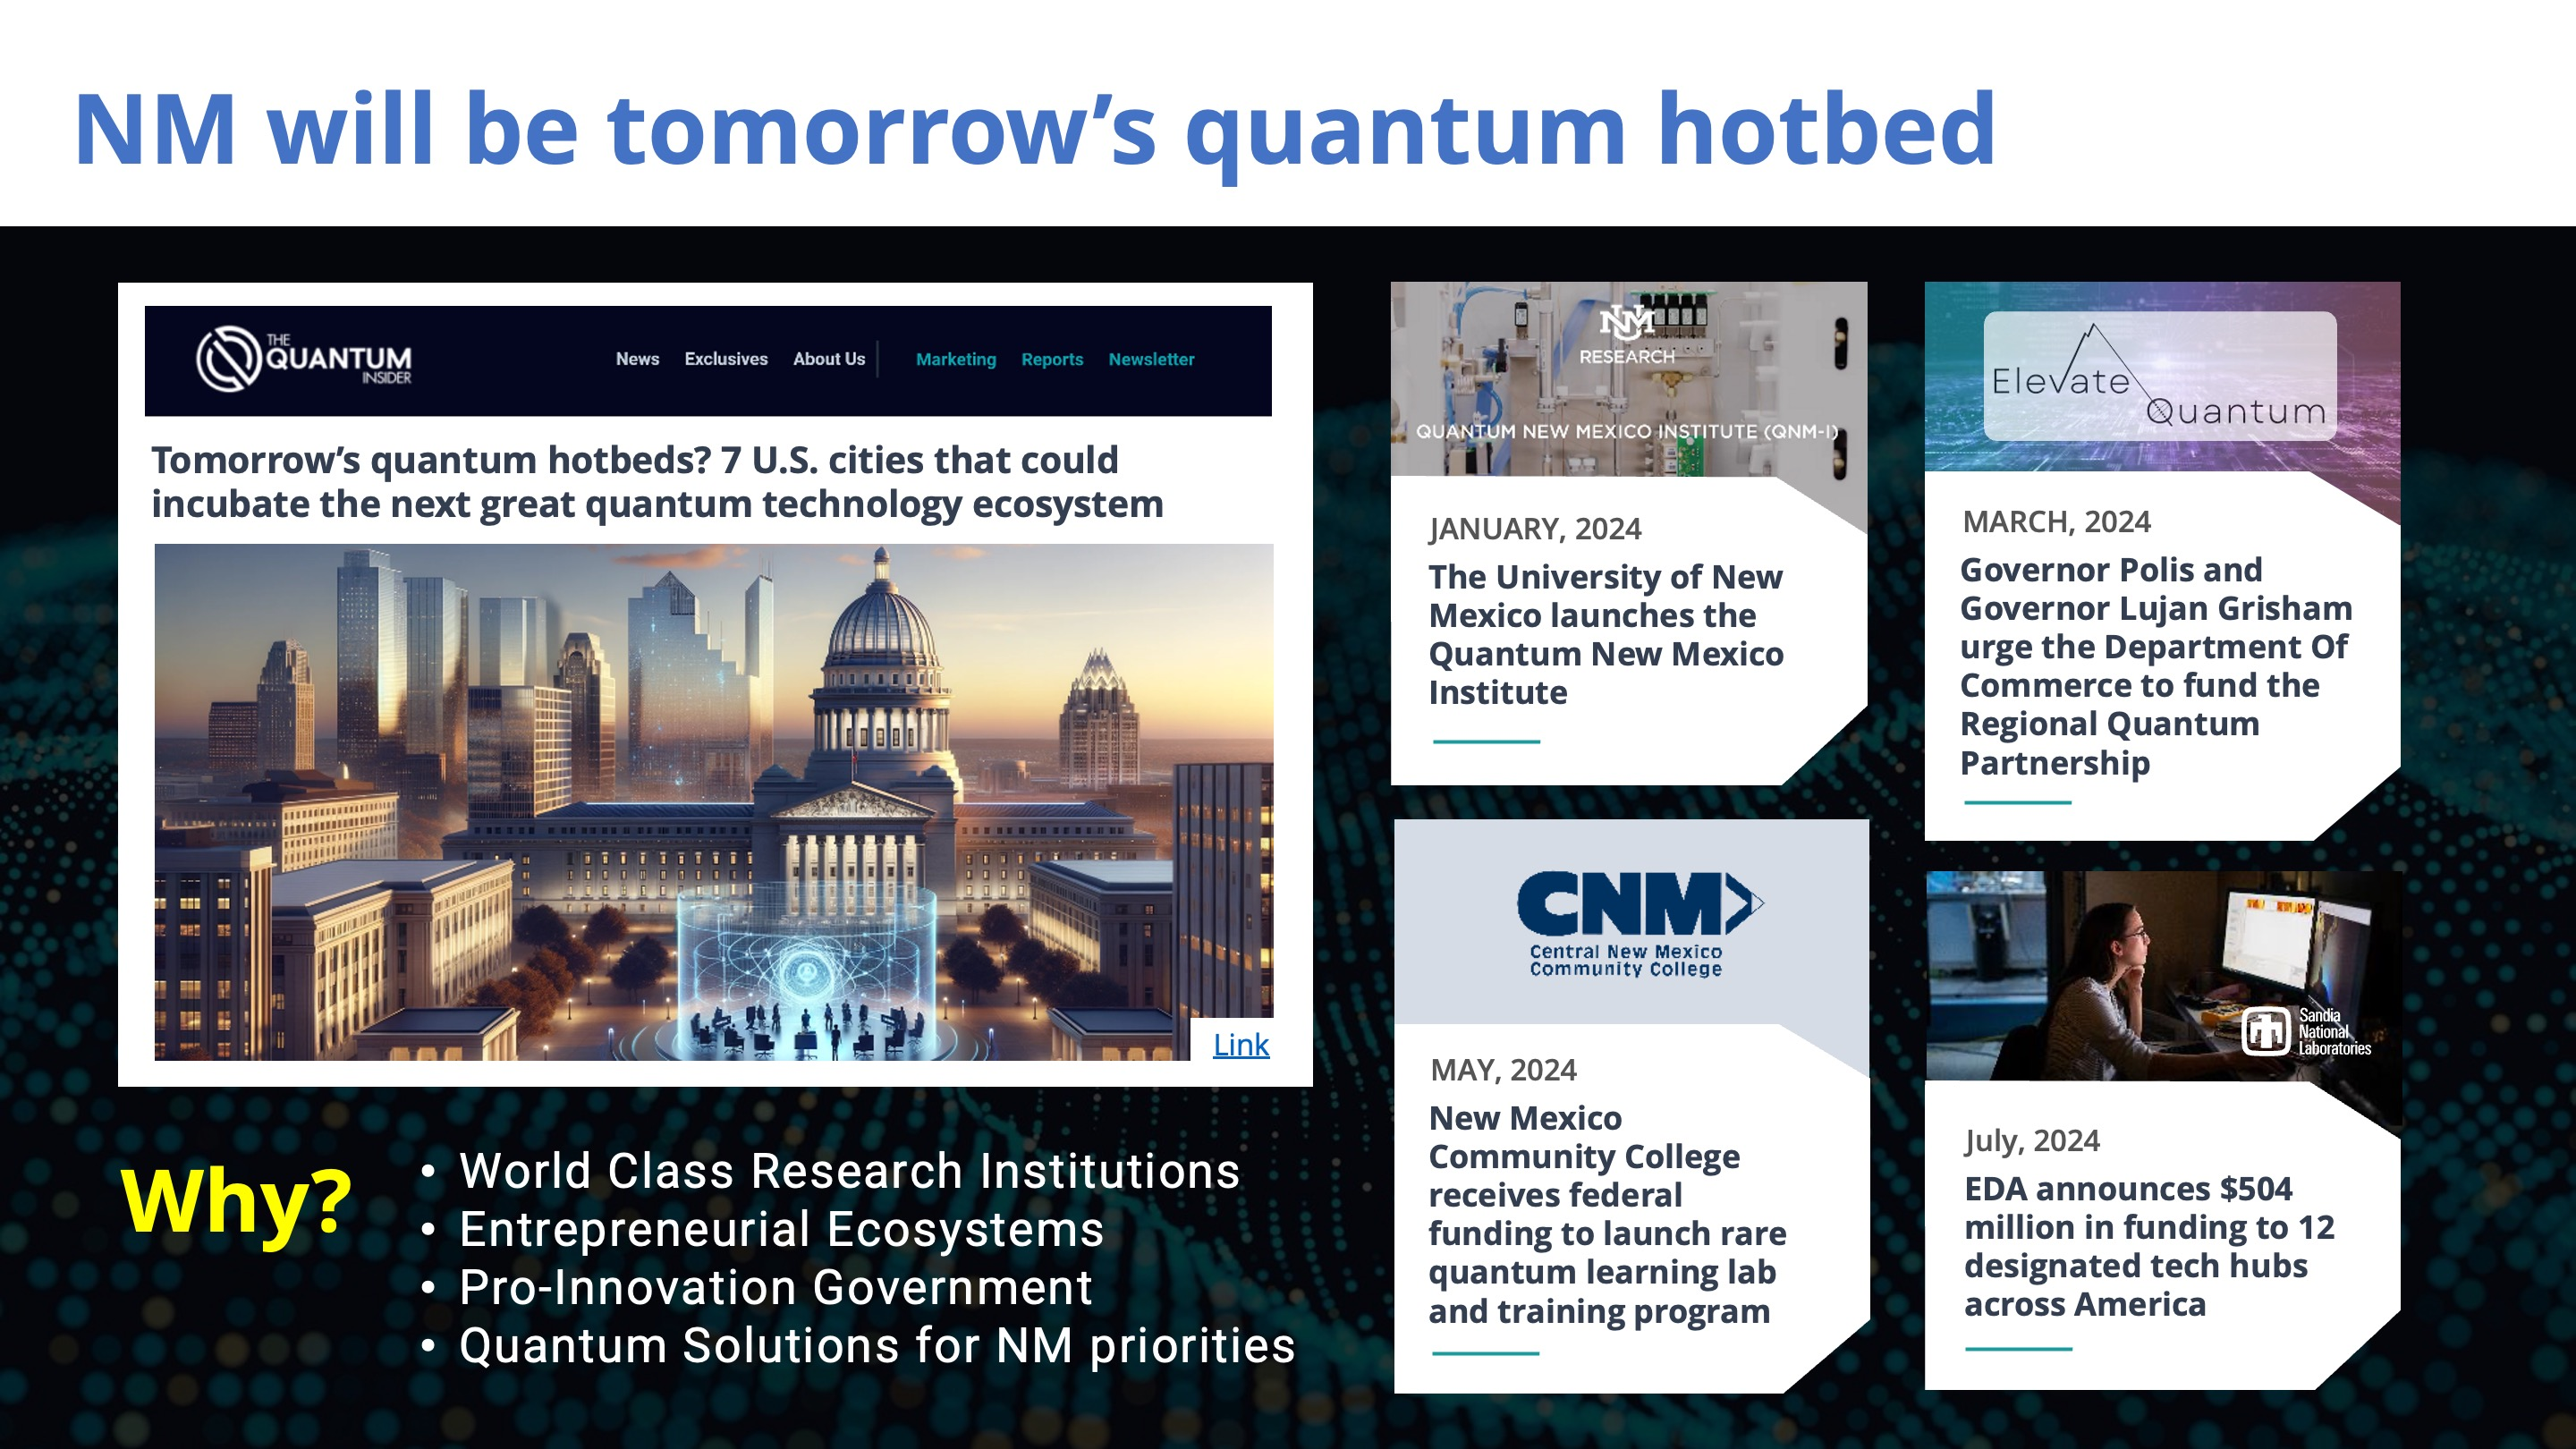
\includegraphics[width=12cm]{fig/Slide2.jpeg}
\end{center}
\end{frame}

\begin{frame}\frametitle{Introduction}
\begin{center}
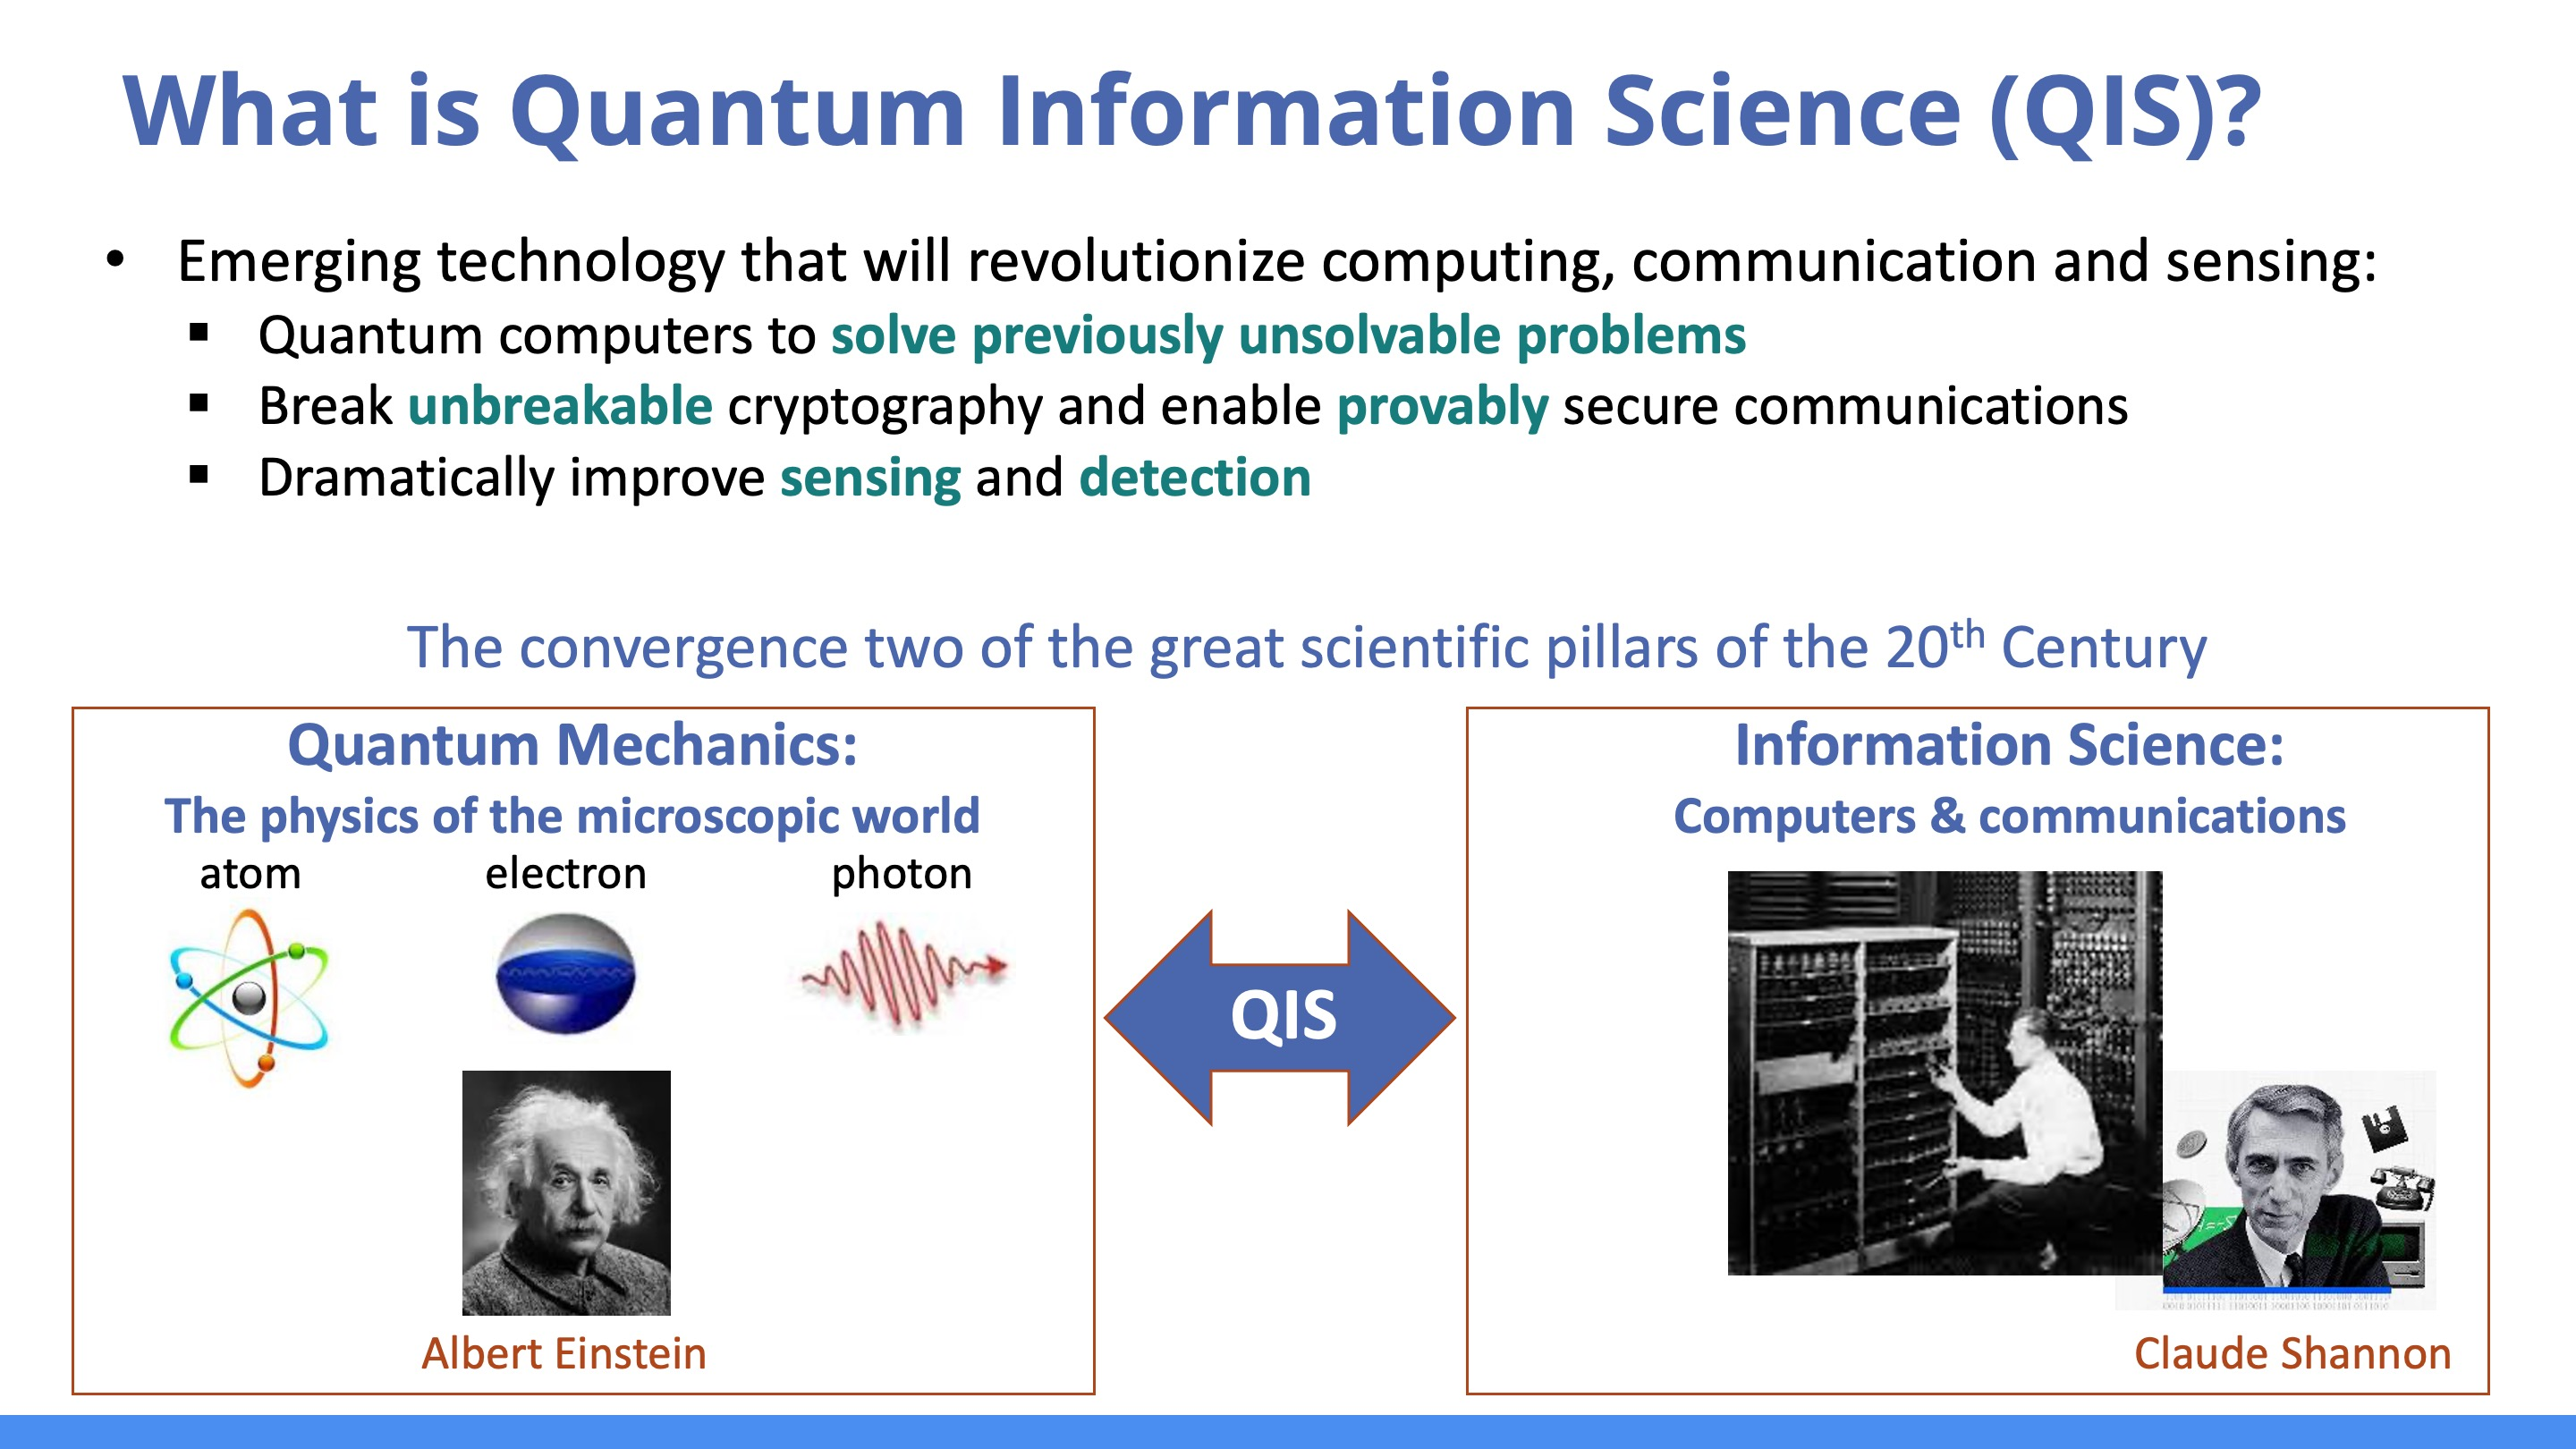
\includegraphics[width=12cm]{fig/Slide4.jpeg}
\end{center}
\end{frame}

\begin{frame}\frametitle{Introduction}
\begin{center}
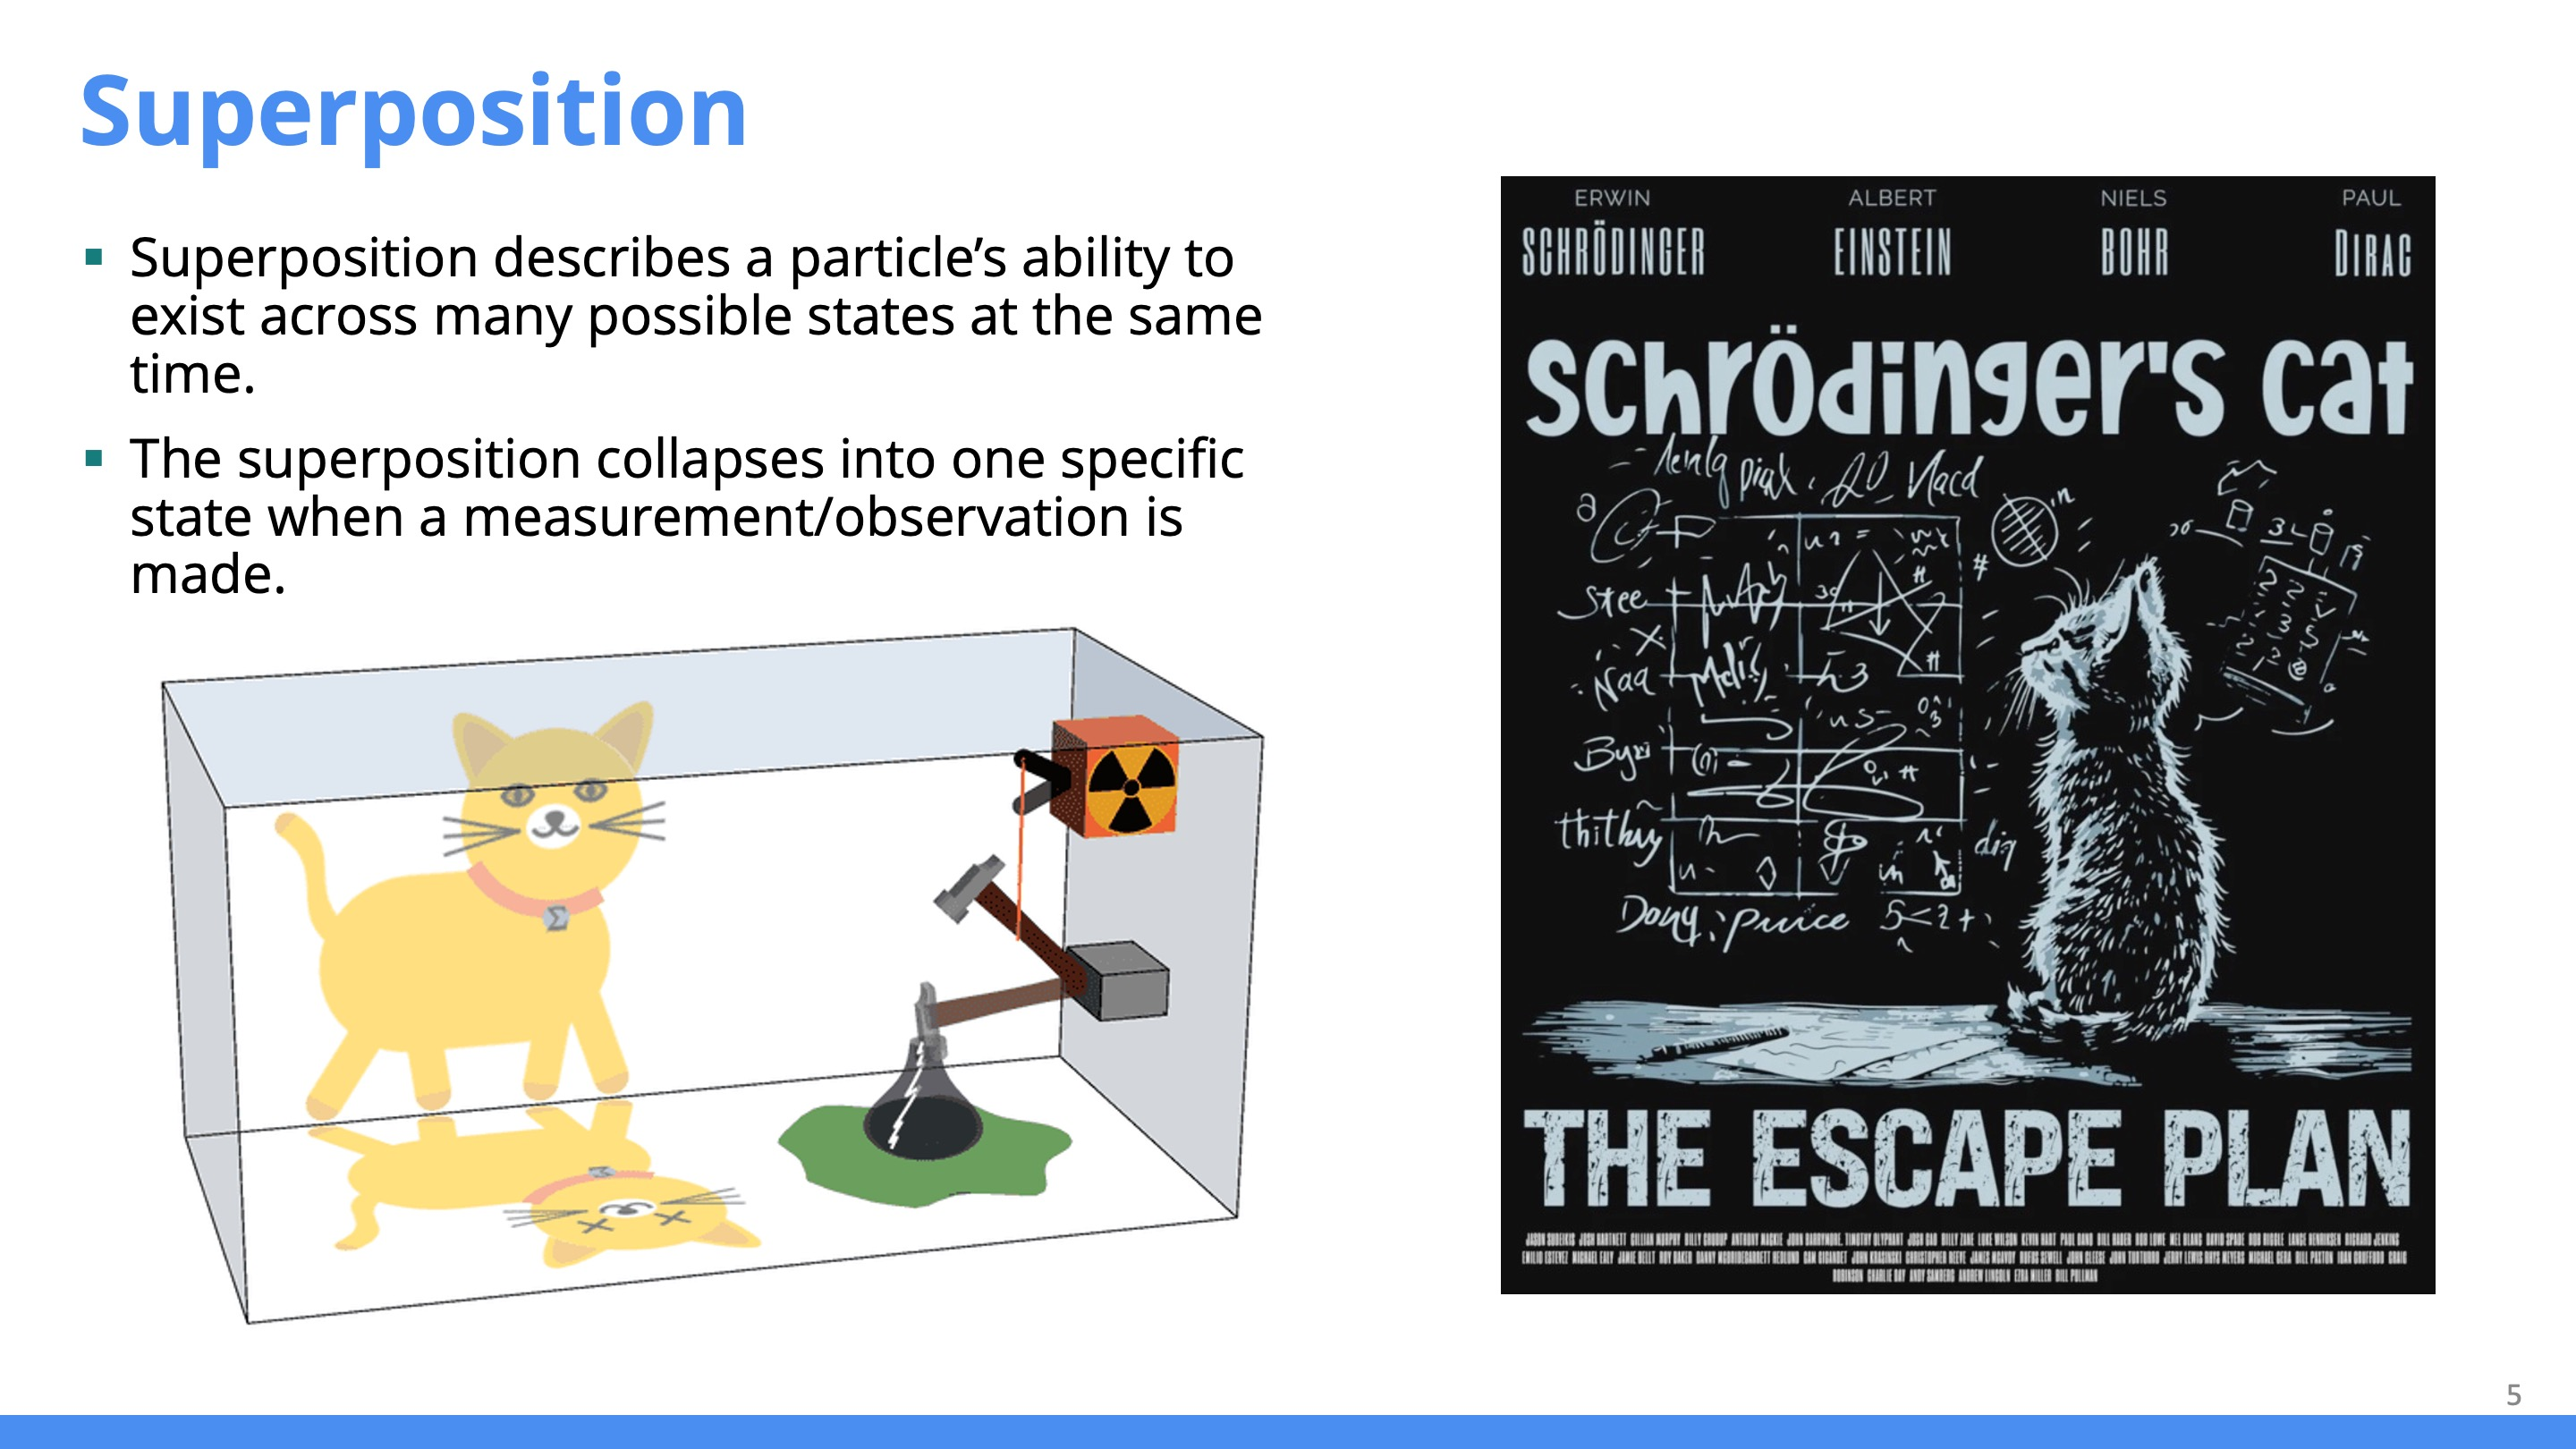
\includegraphics[width=12cm]{fig/supercat.jpg}
\end{center}
\end{frame}

\begin{frame}\frametitle{Introduction}
\begin{center}
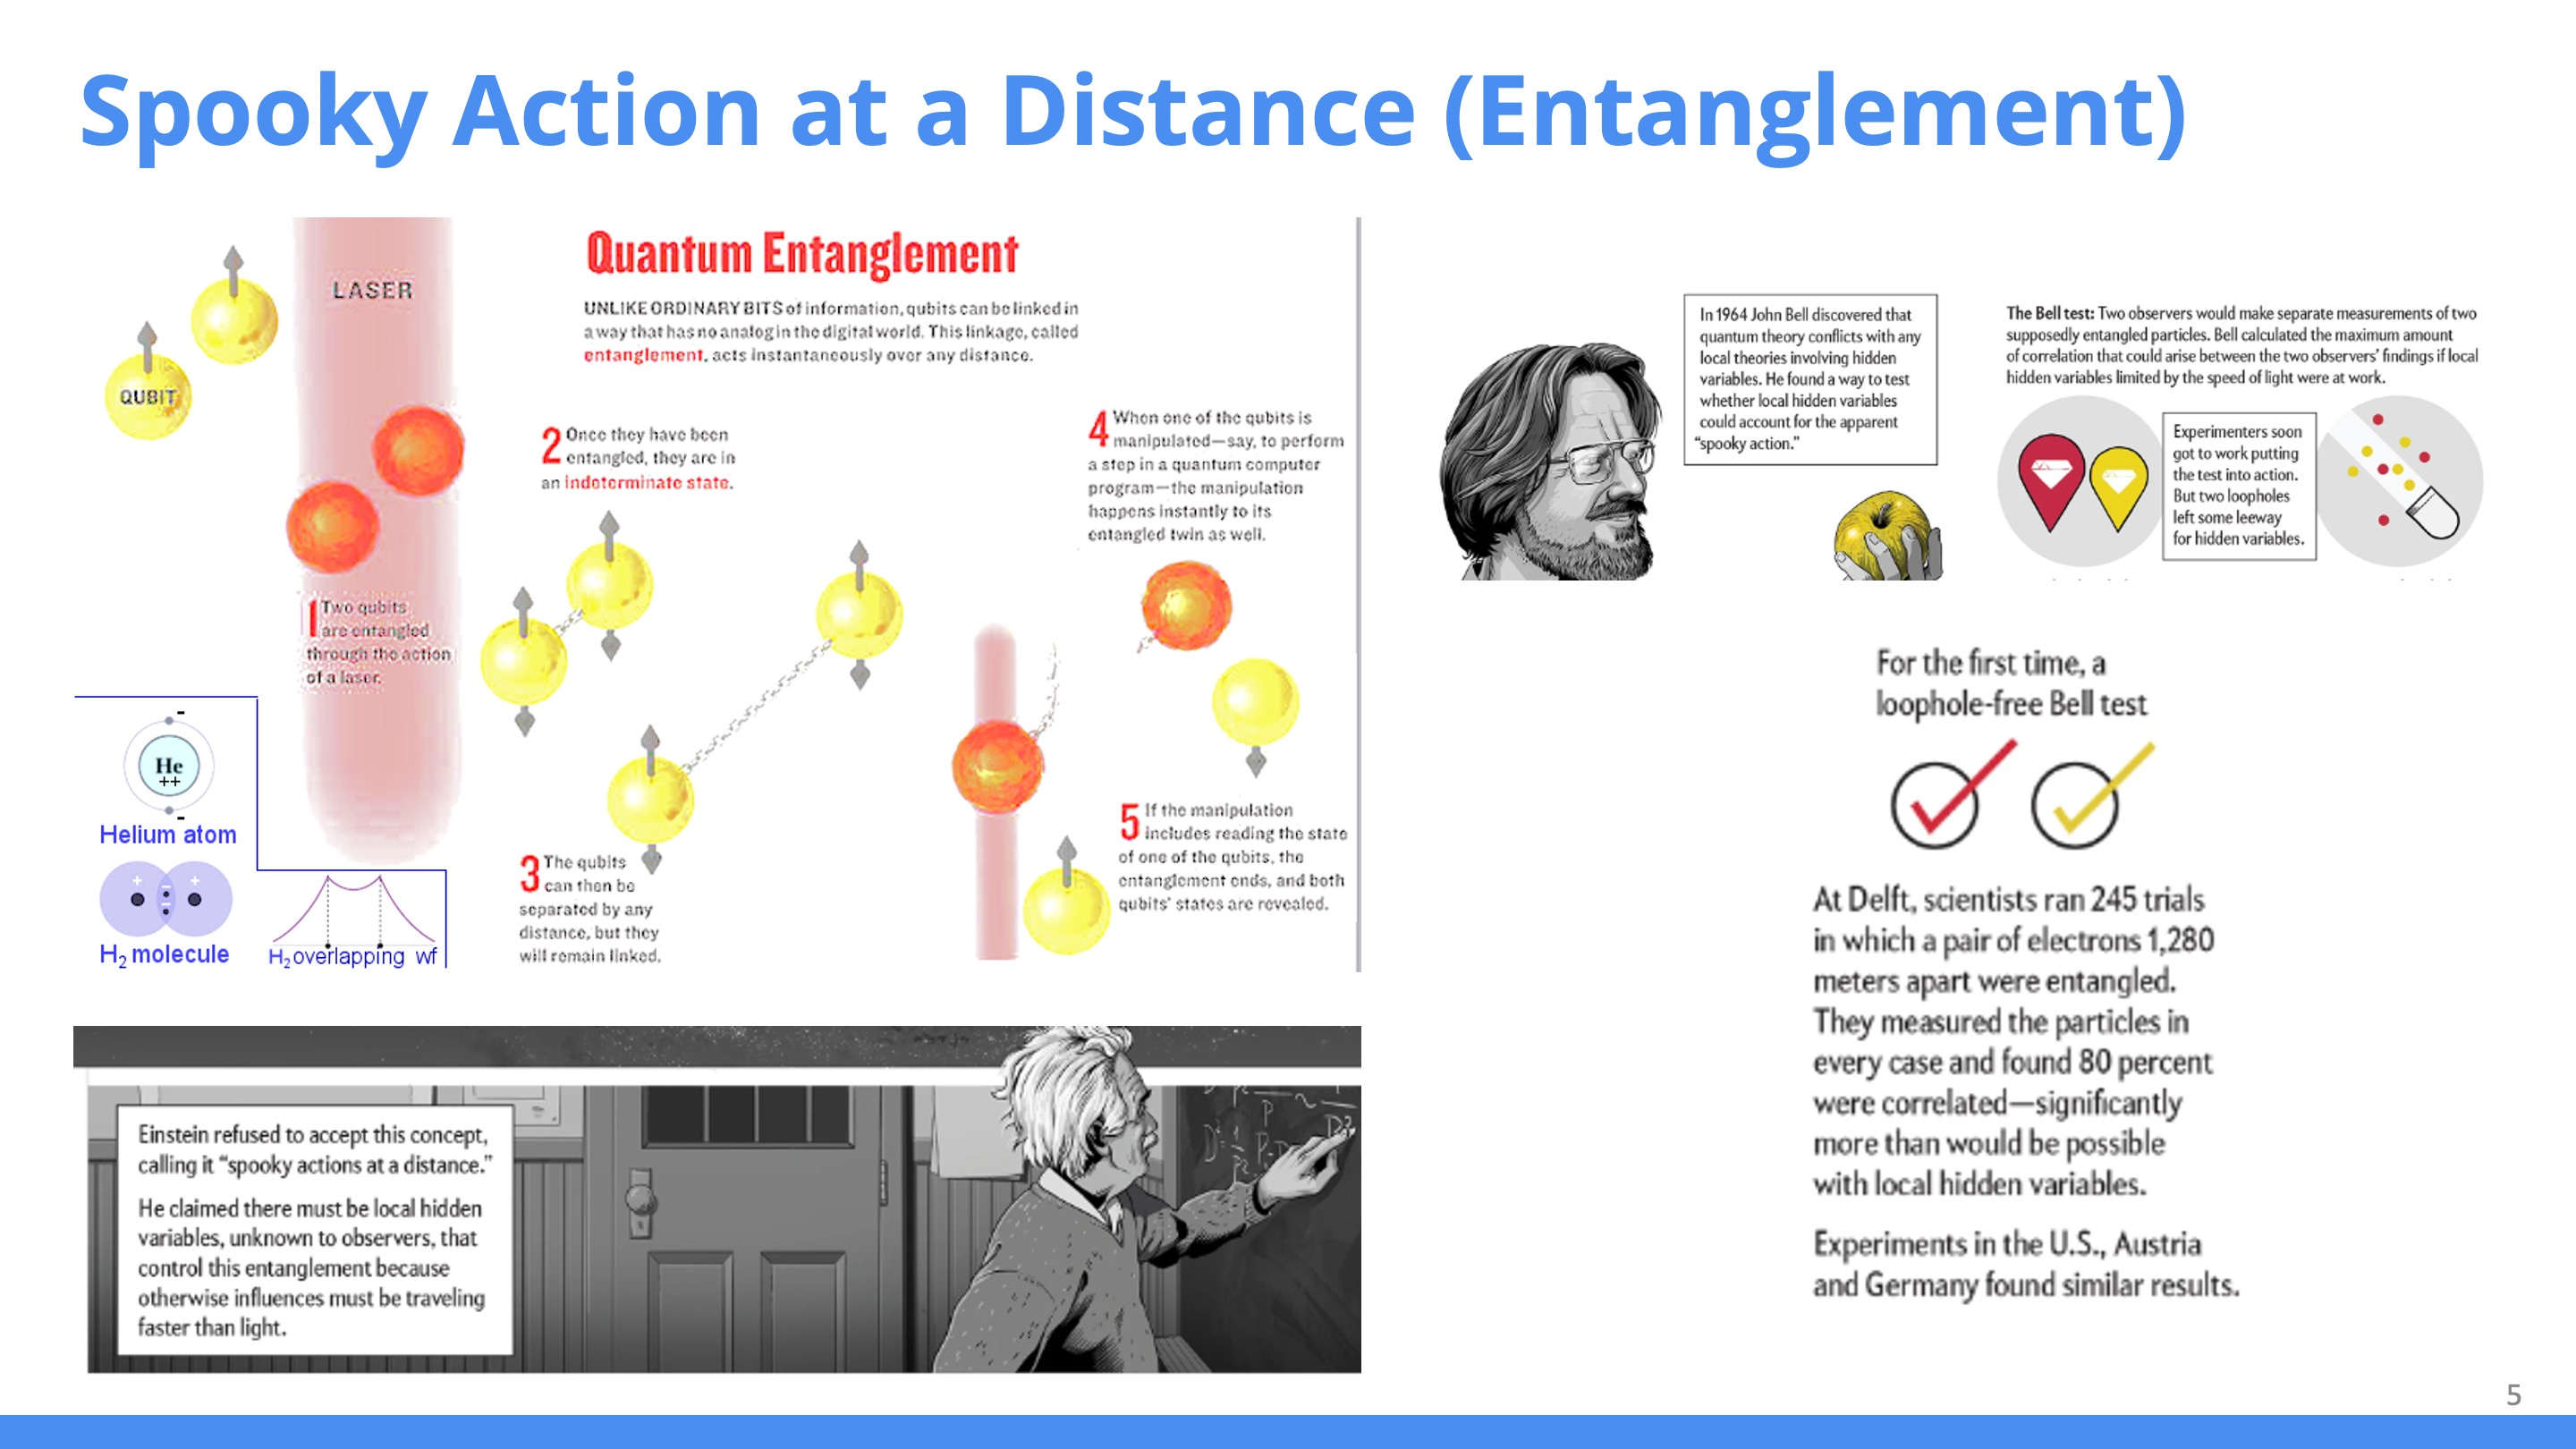
\includegraphics[width=12cm]{fig/Slide5.jpeg}
\end{center}
\end{frame}

\begin{frame}\frametitle{Introduction}
\begin{center}
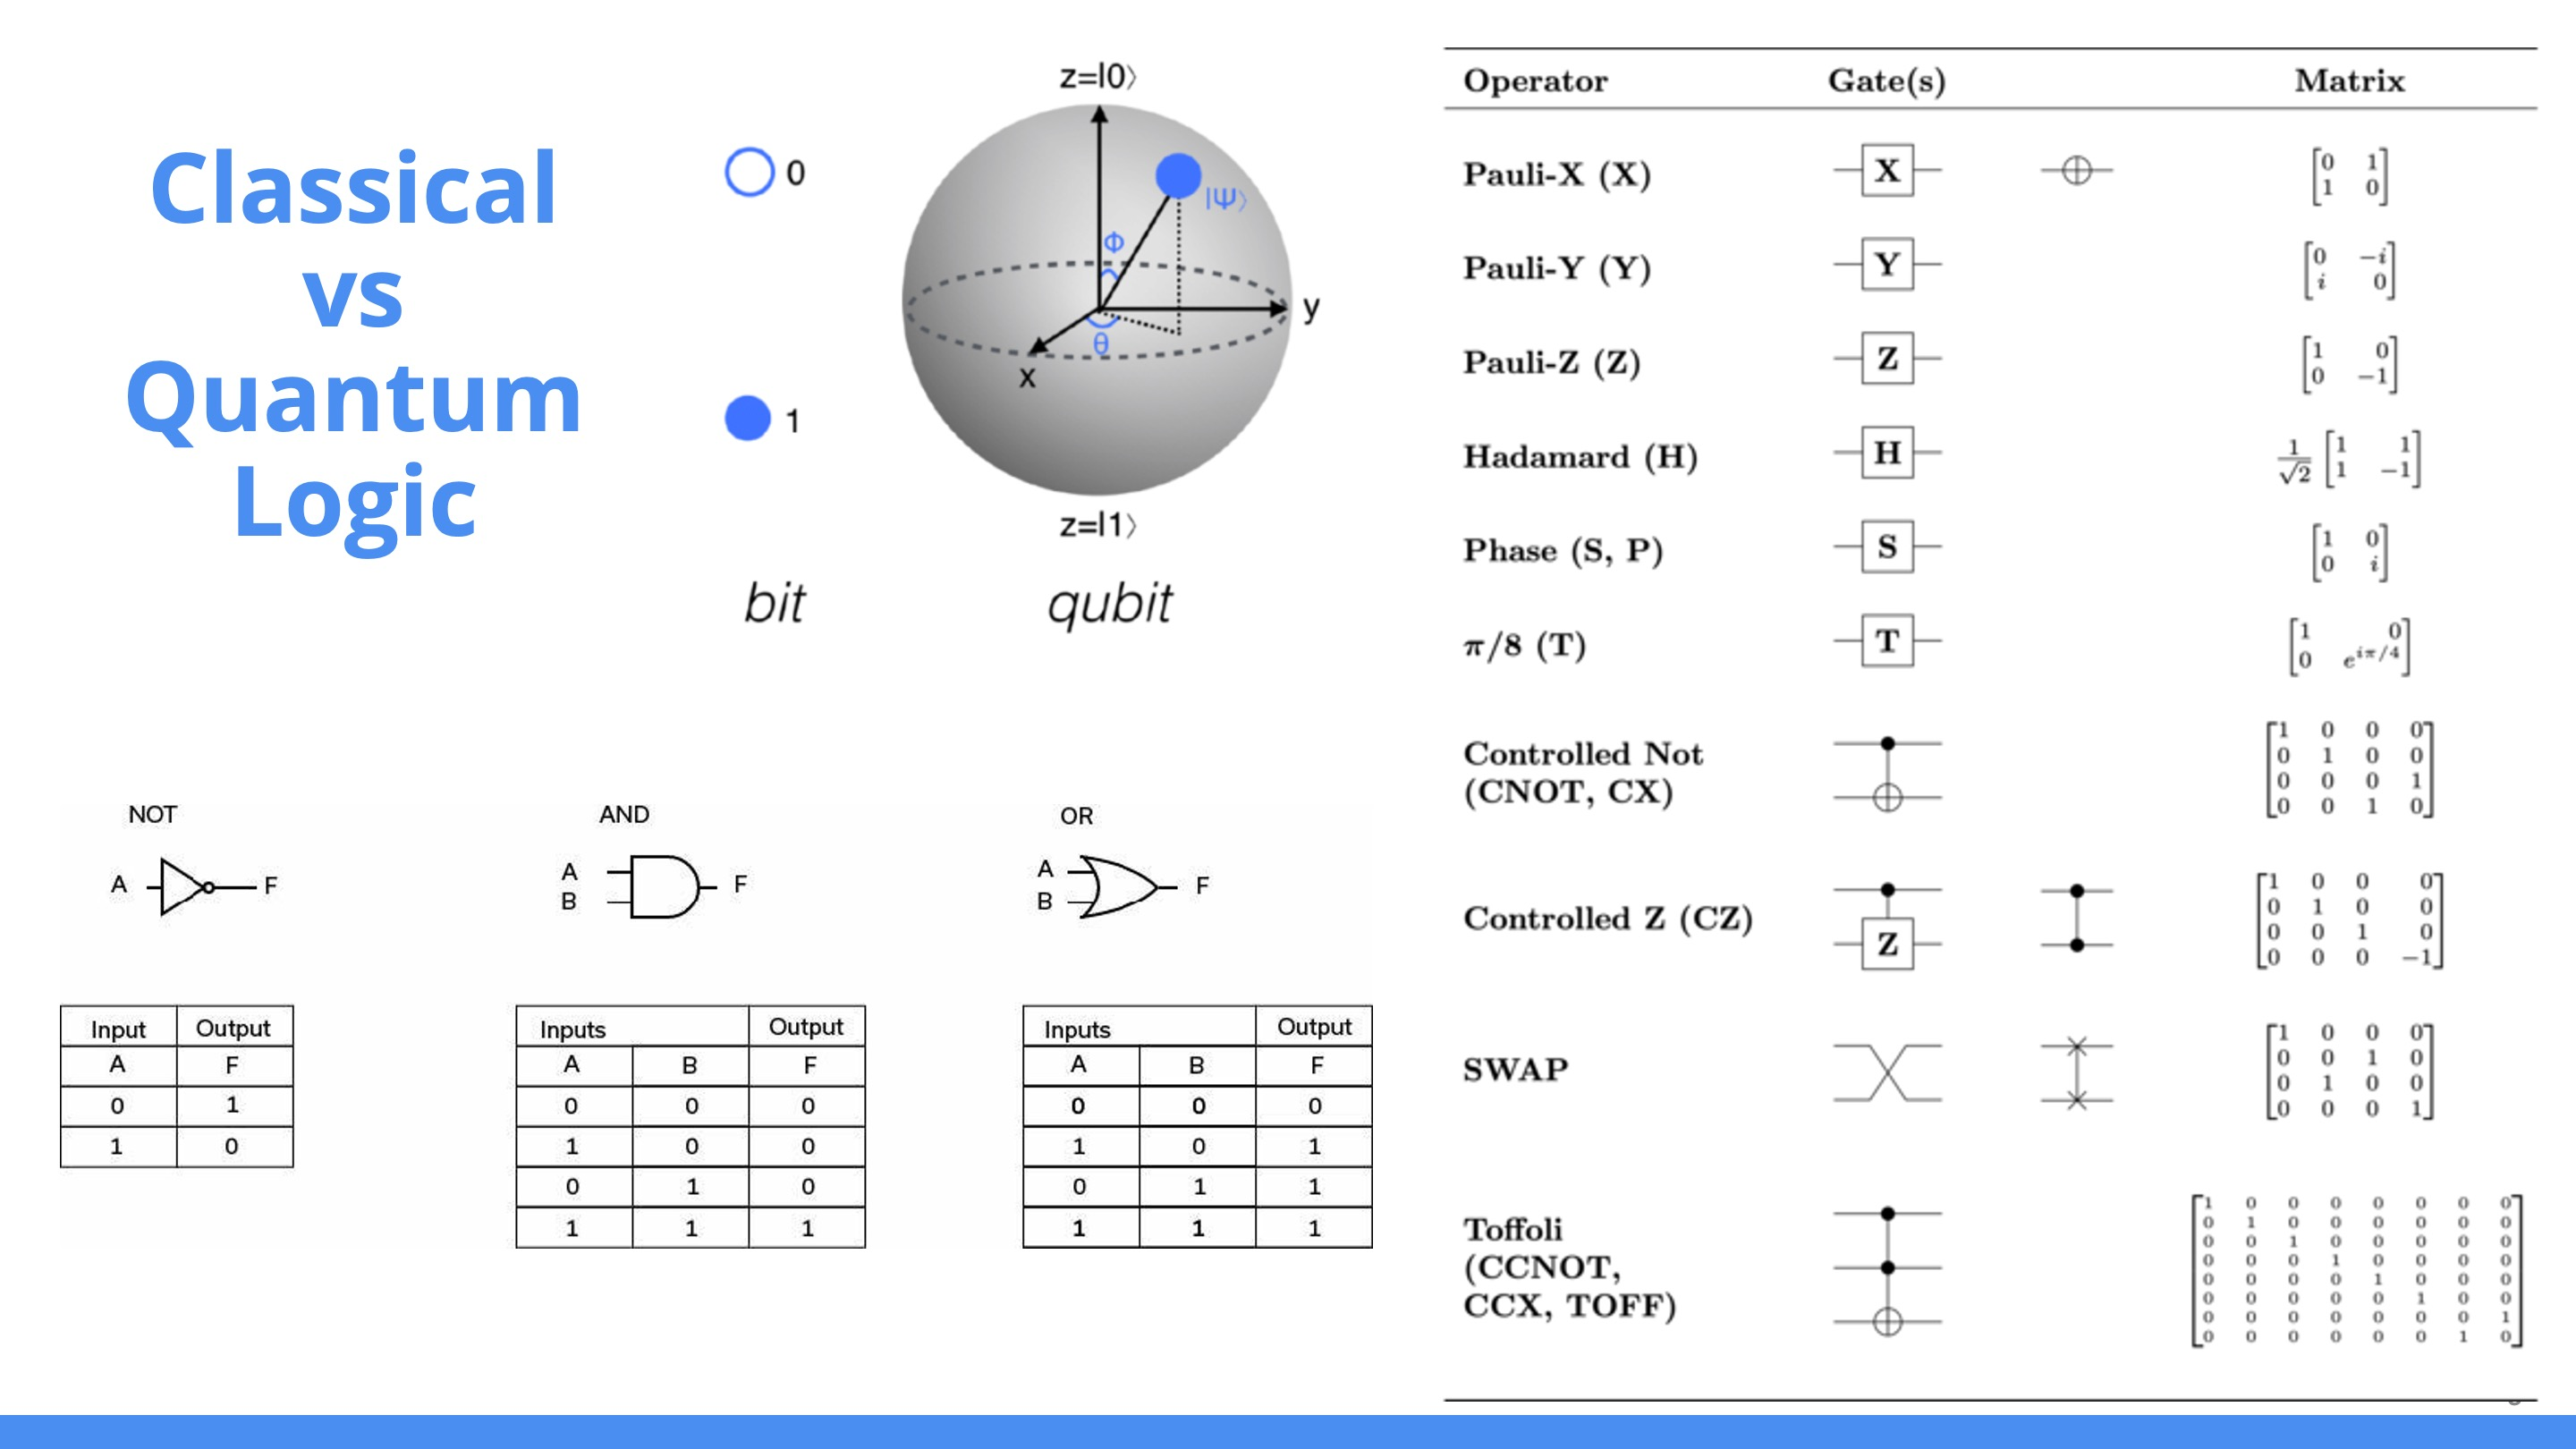
\includegraphics[width=12cm]{fig/Slide6.jpeg}
\end{center}
\end{frame}

\begin{frame}\frametitle{Introduction}
\begin{center}
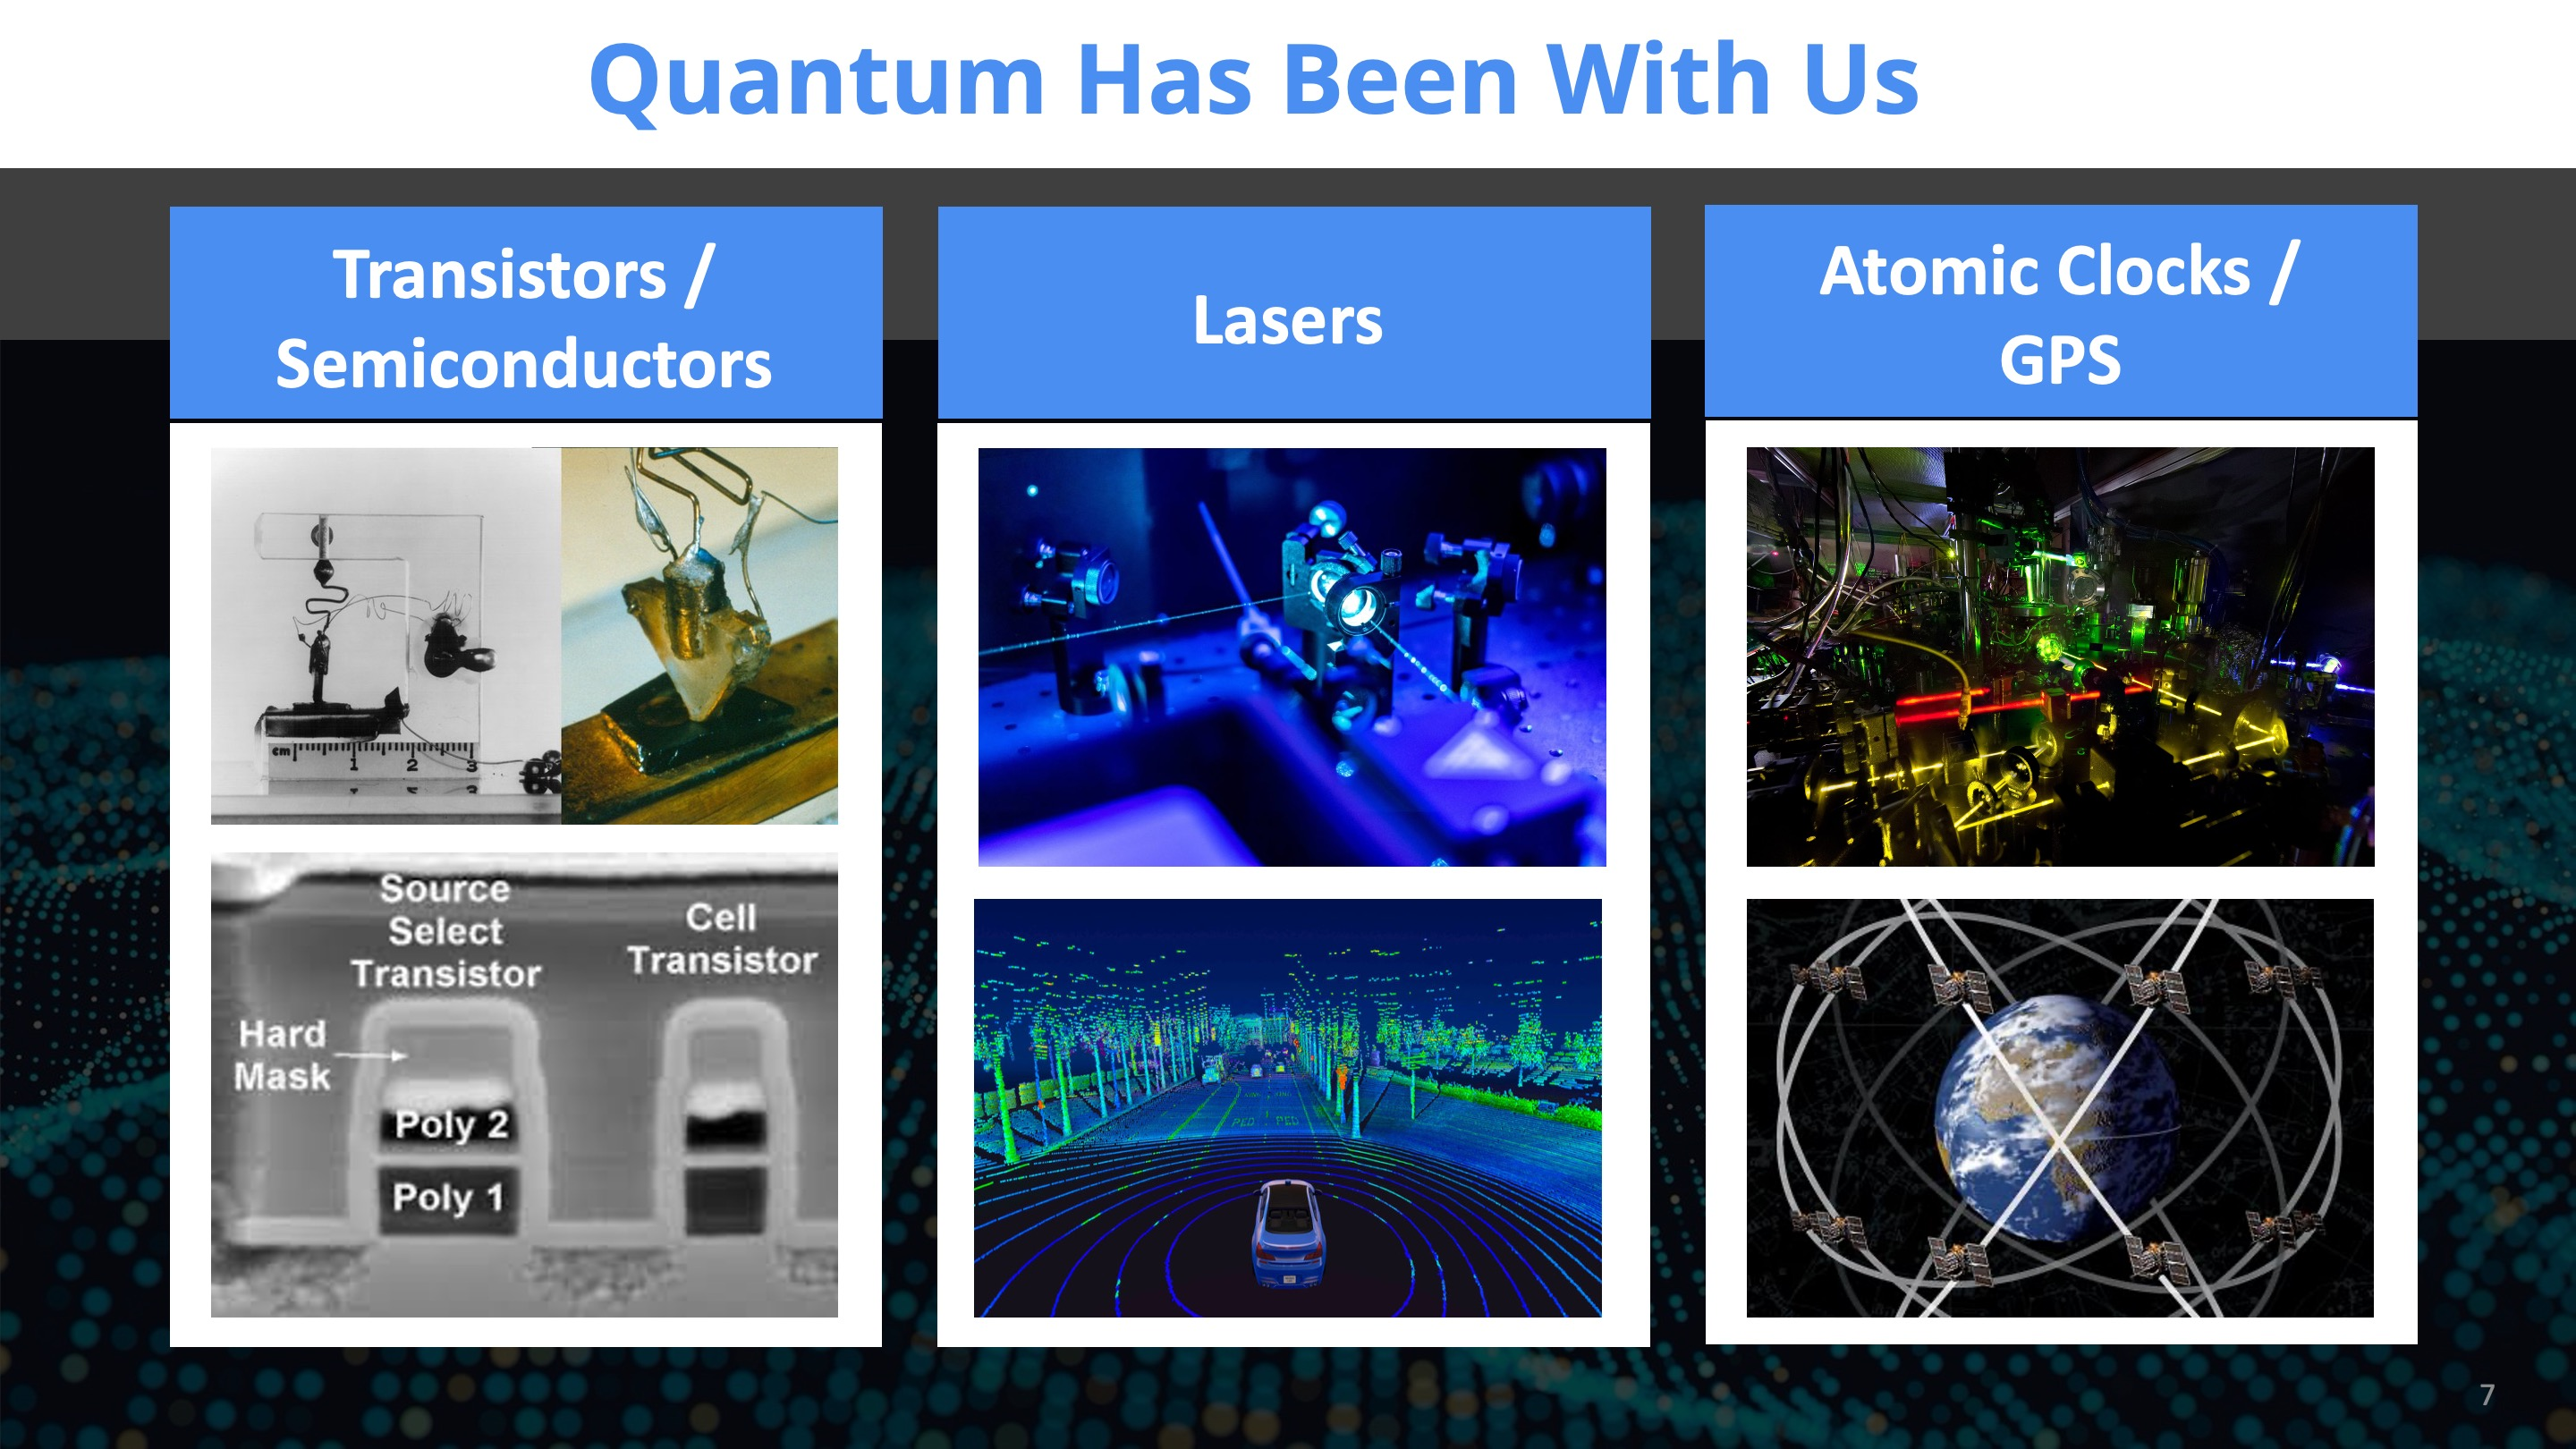
\includegraphics[width=12cm]{fig/Slide7.jpeg}
\end{center}
\end{frame}

\begin{frame}\frametitle{Introduction}
\begin{center}
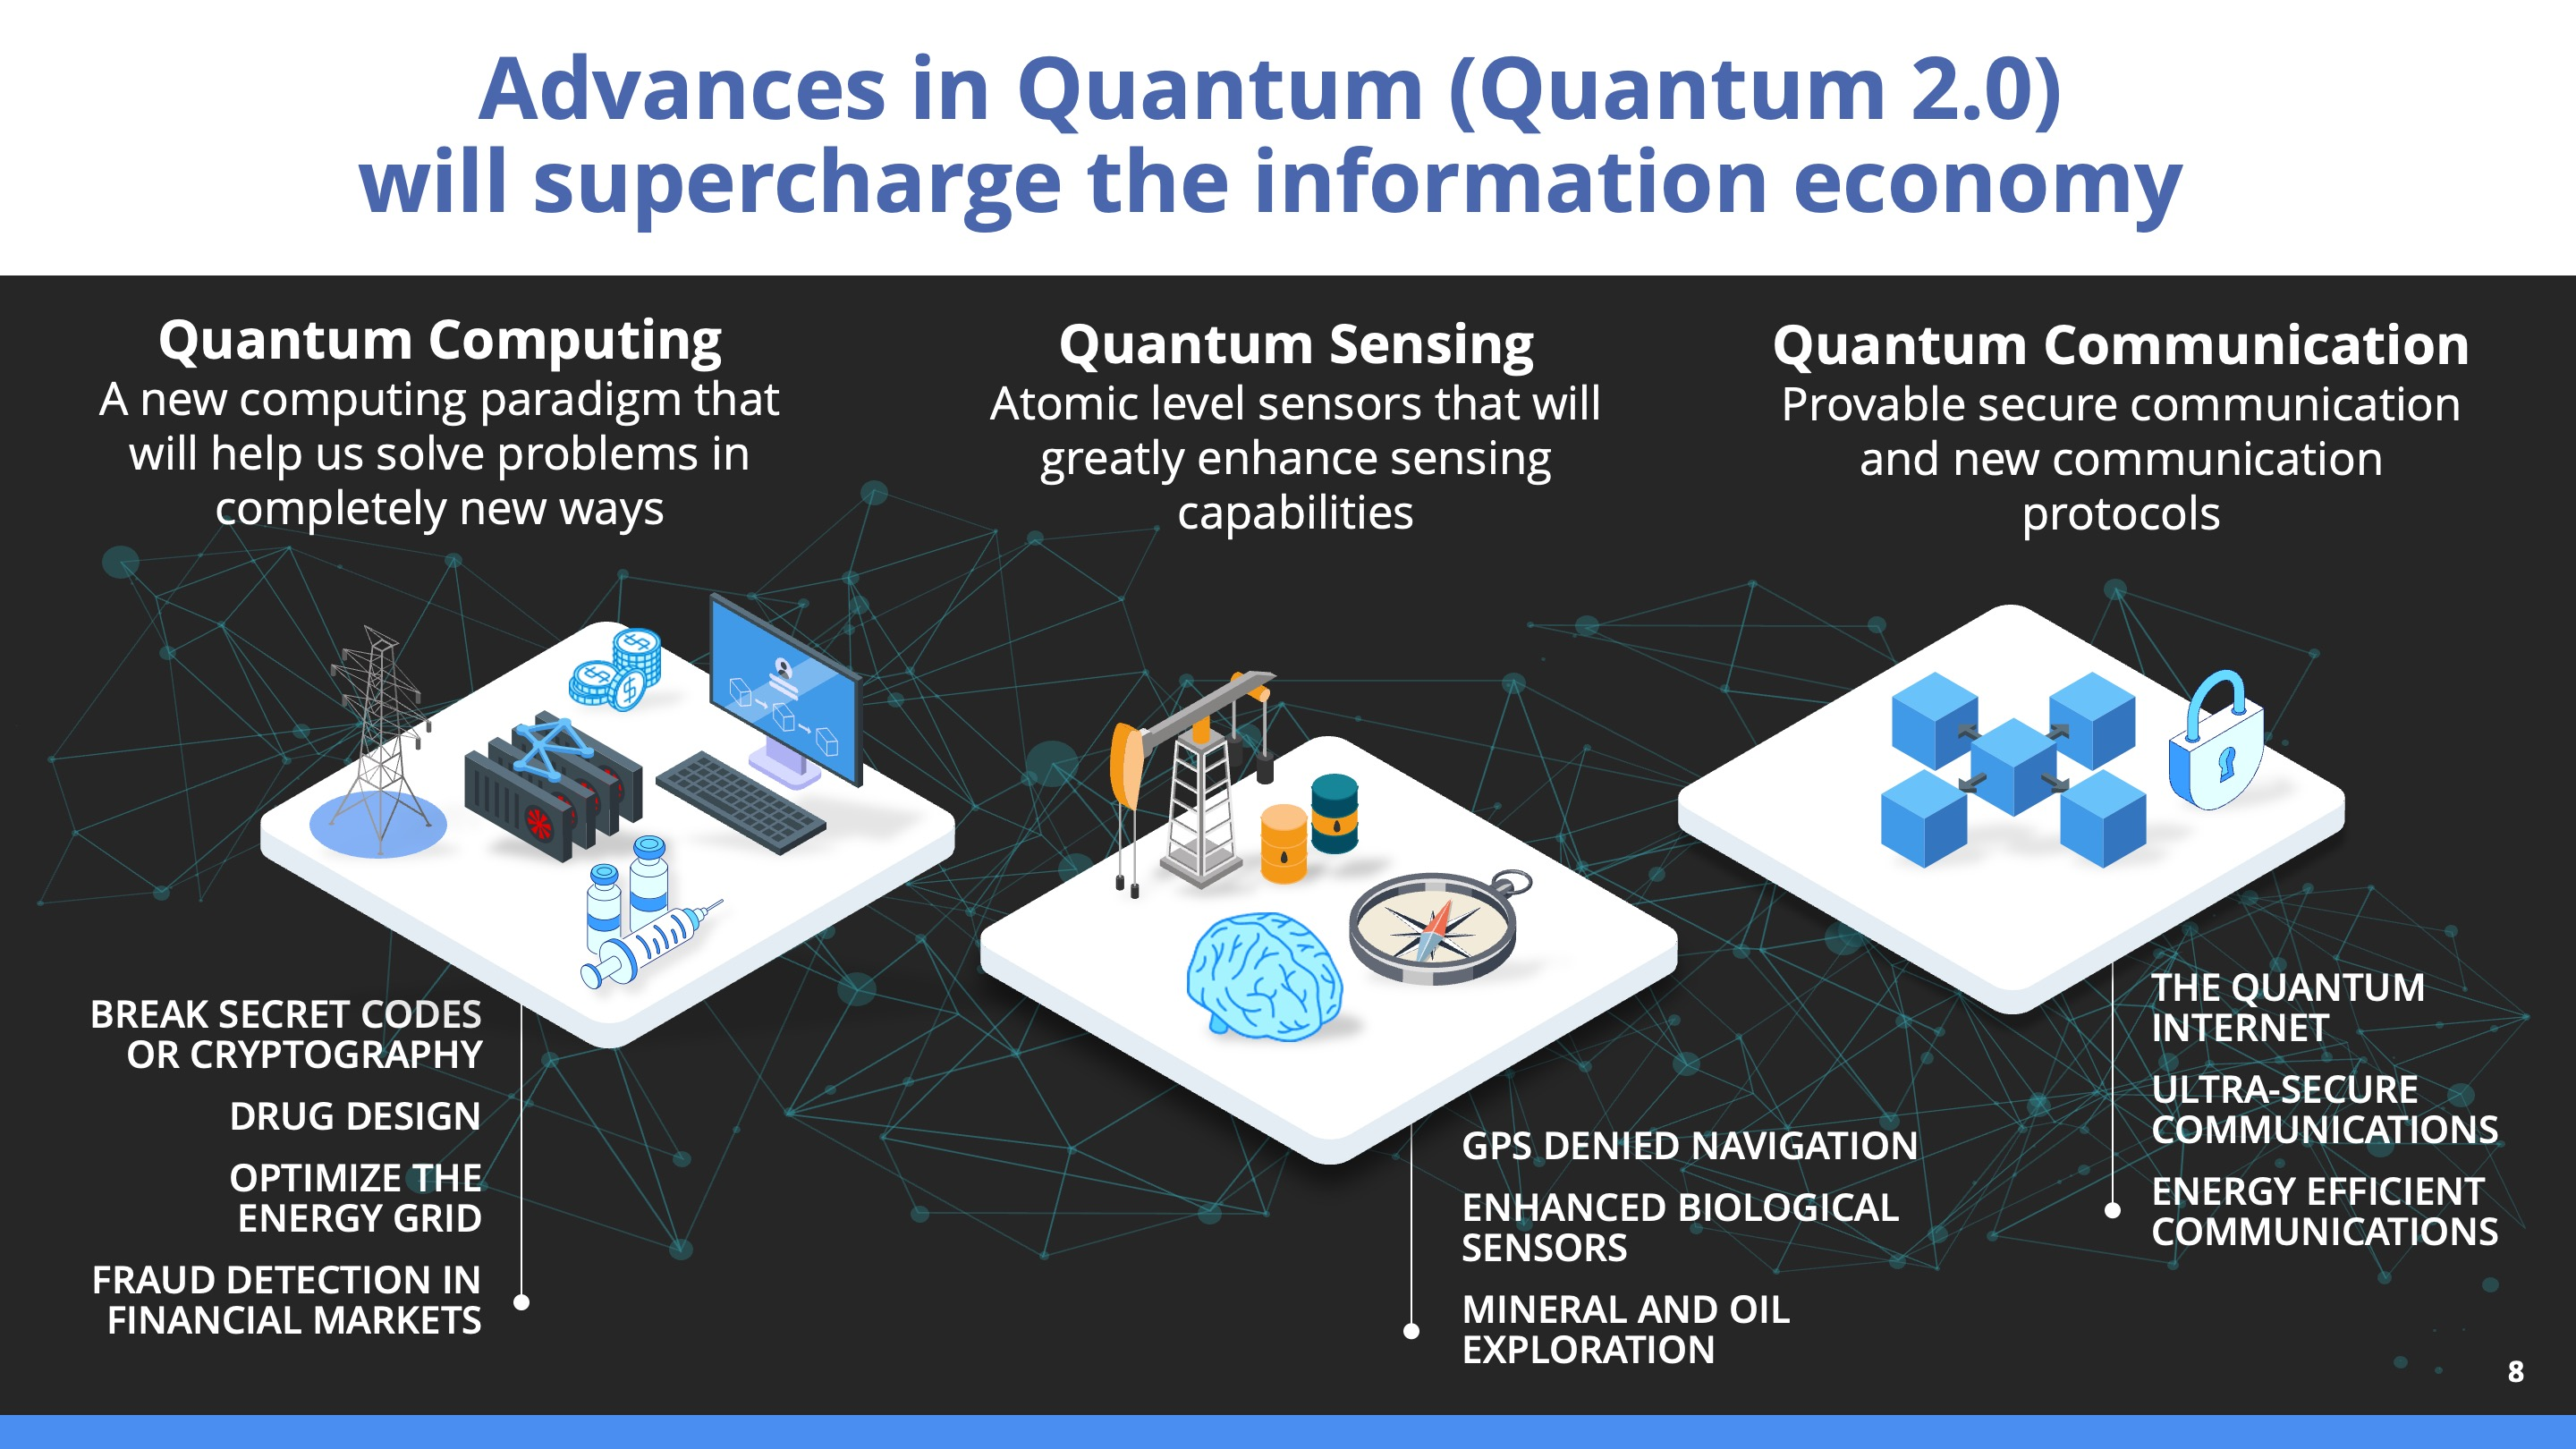
\includegraphics[width=12cm]{fig/Slide8.jpeg}
\end{center}
\end{frame}

\begin{frame}\frametitle{Introduction}
\begin{center}

\includegraphics[width=12cm]{fig/Slide9.jpeg}
\end{center}
\end{frame}

\begin{frame}\frametitle{Introduction}
\begin{center}
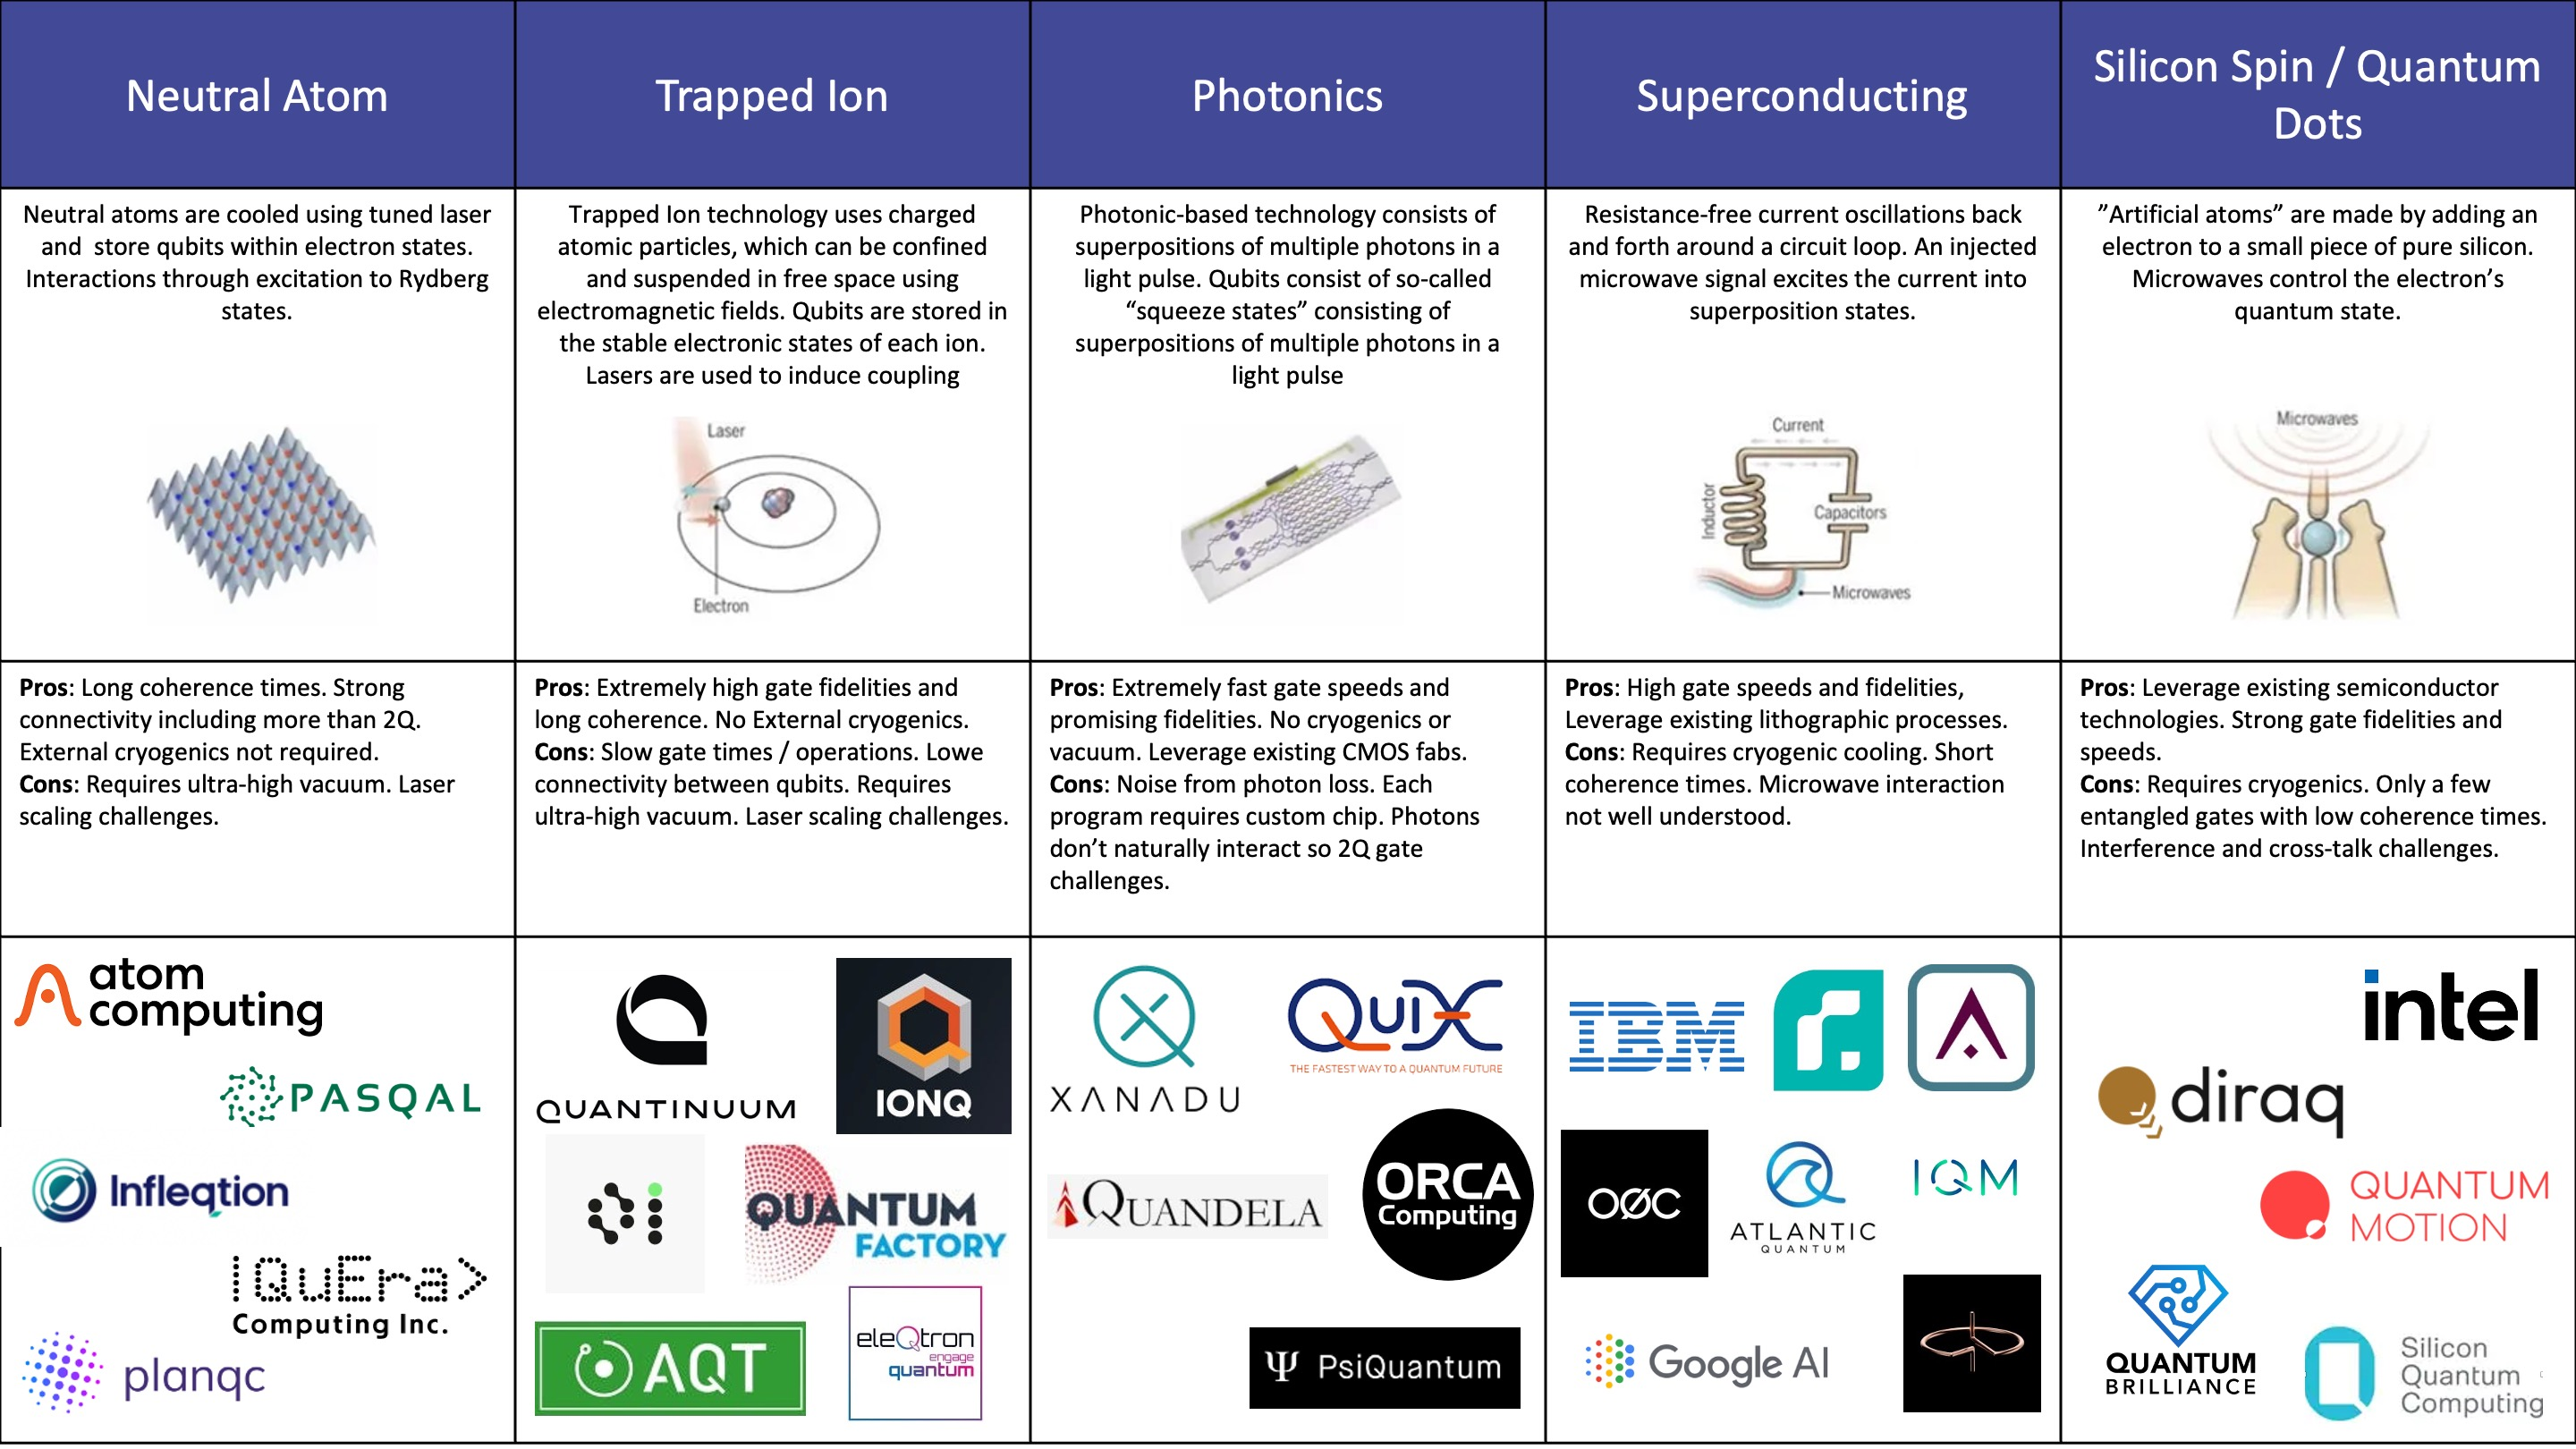
\includegraphics[width=12cm]{fig/Slide10.jpeg}
\end{center}
\end{frame}

\begin{frame}\frametitle{Introduction}
\begin{center}
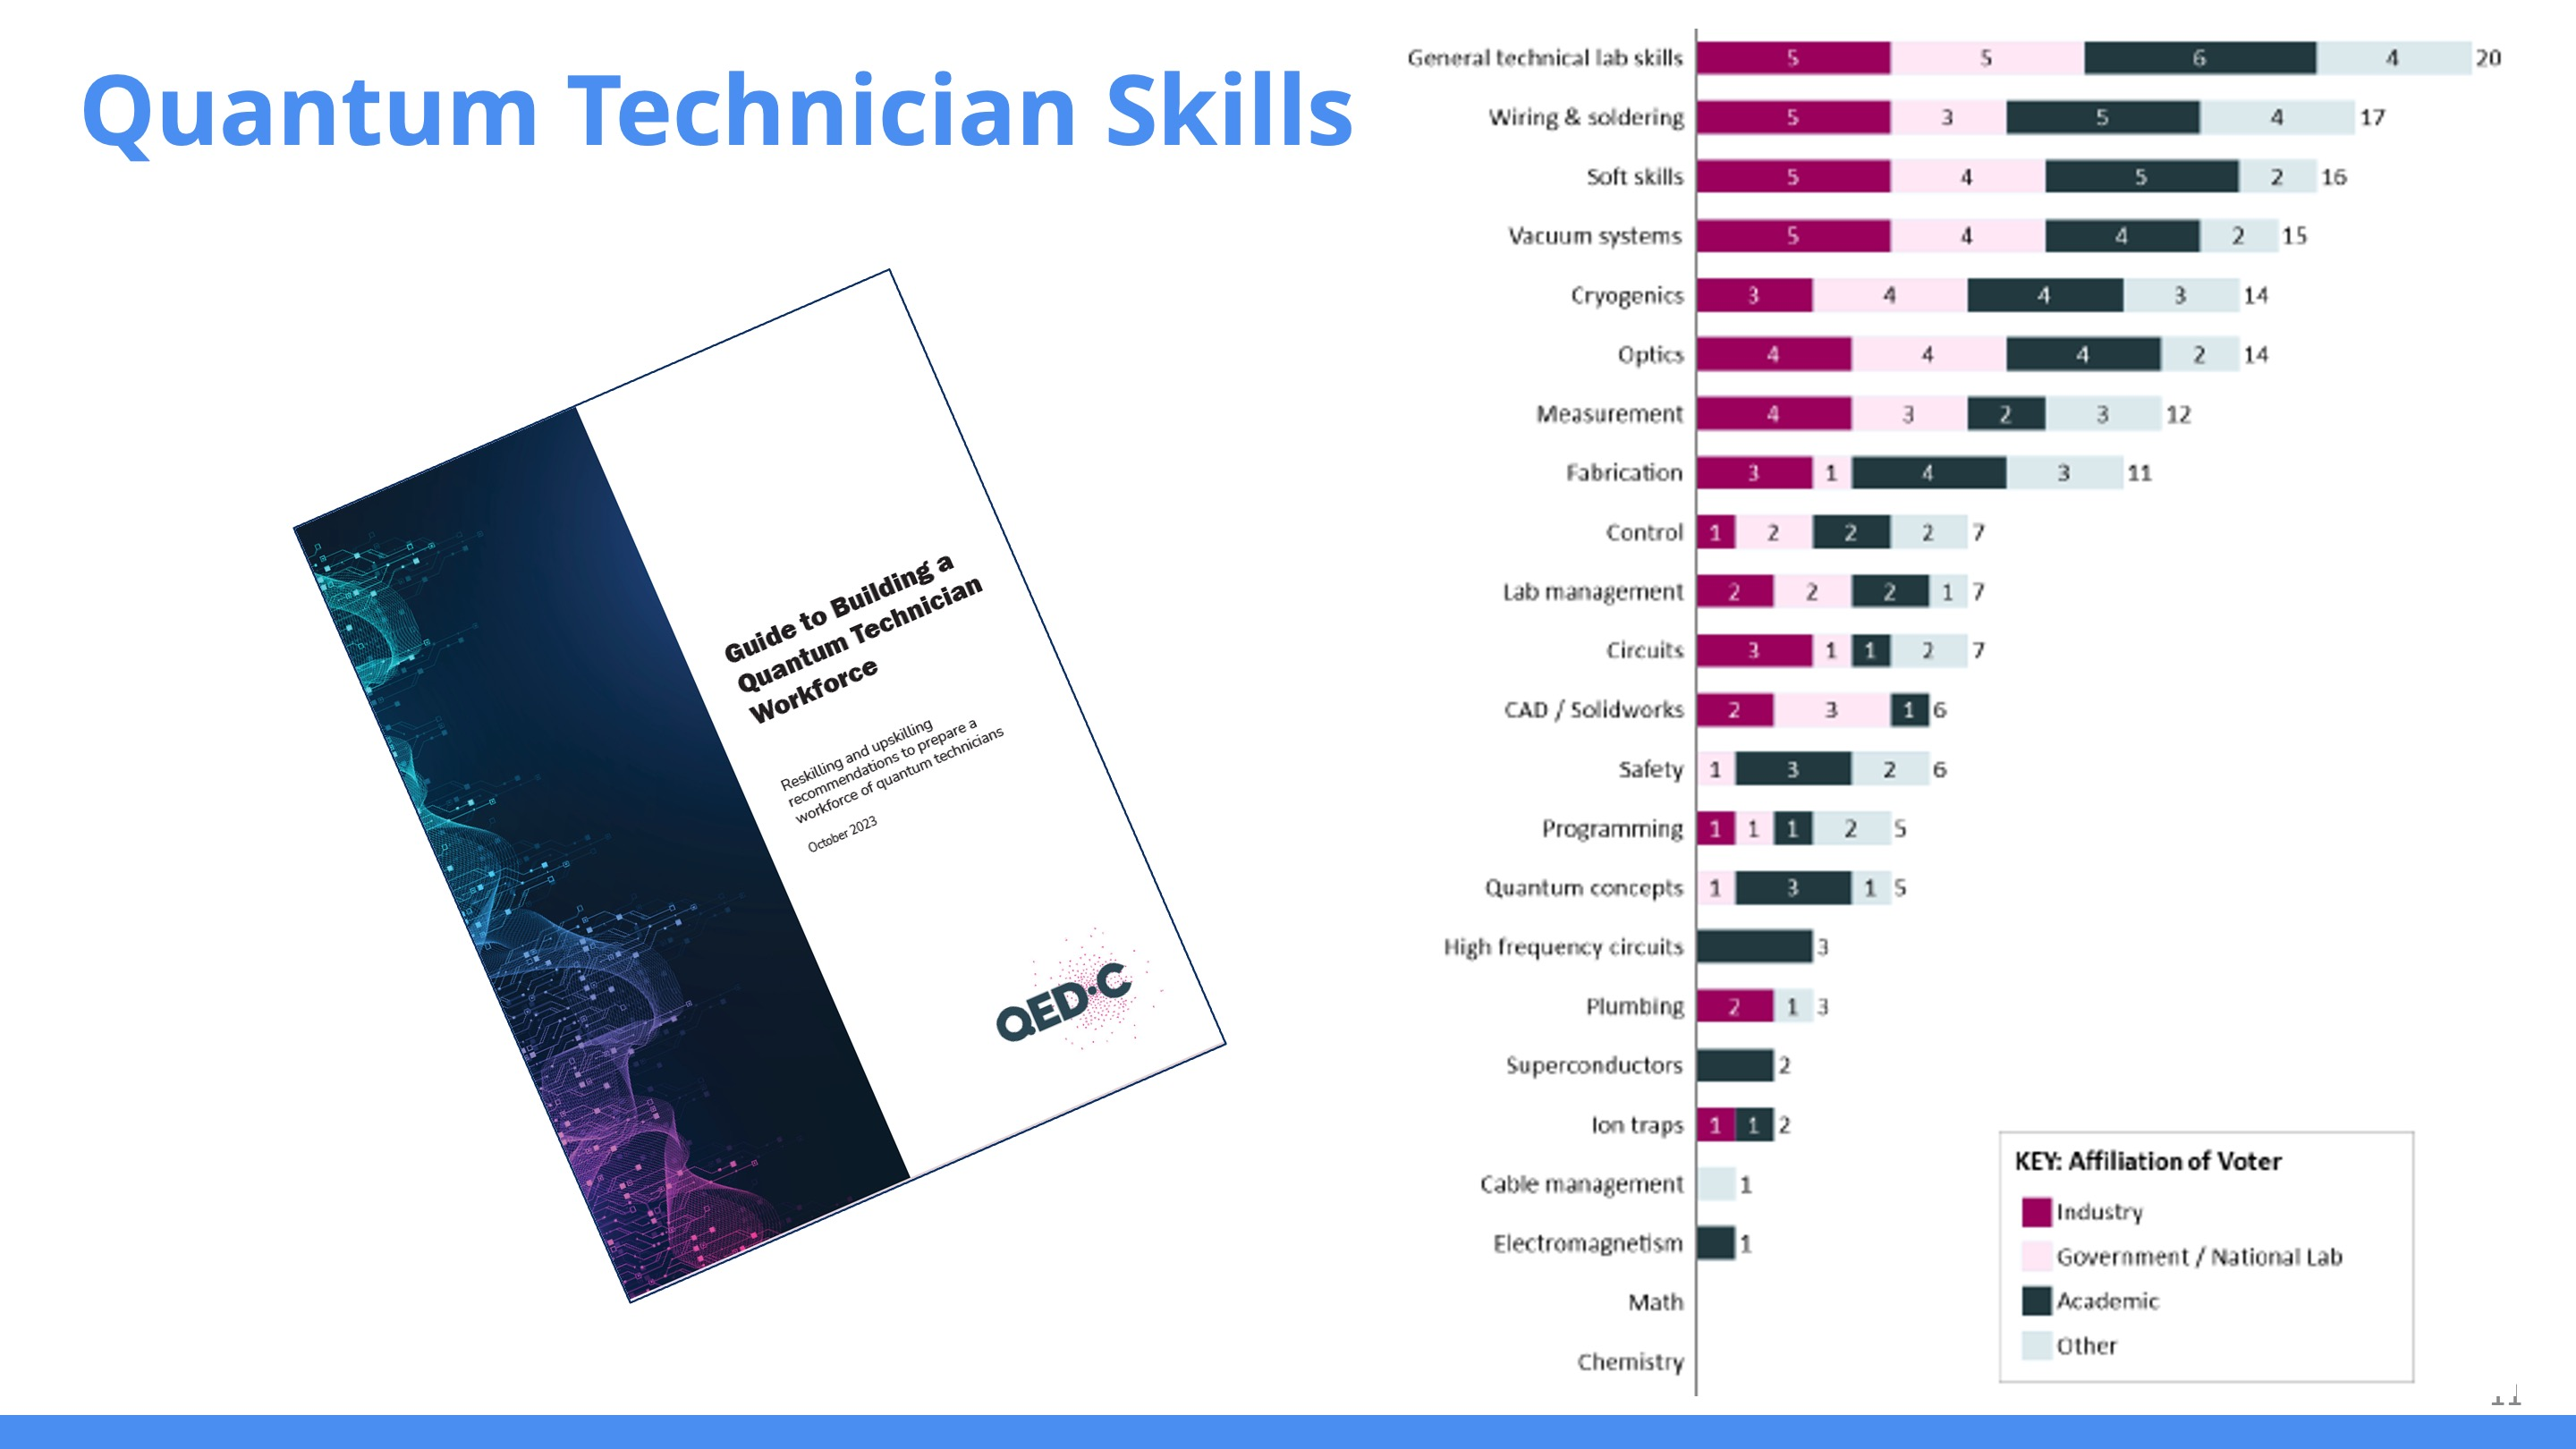
\includegraphics[width=12cm]{fig/Slide11.jpeg}
\end{center}
\end{frame}

\begin{frame}\frametitle{Introduction}
\begin{center}
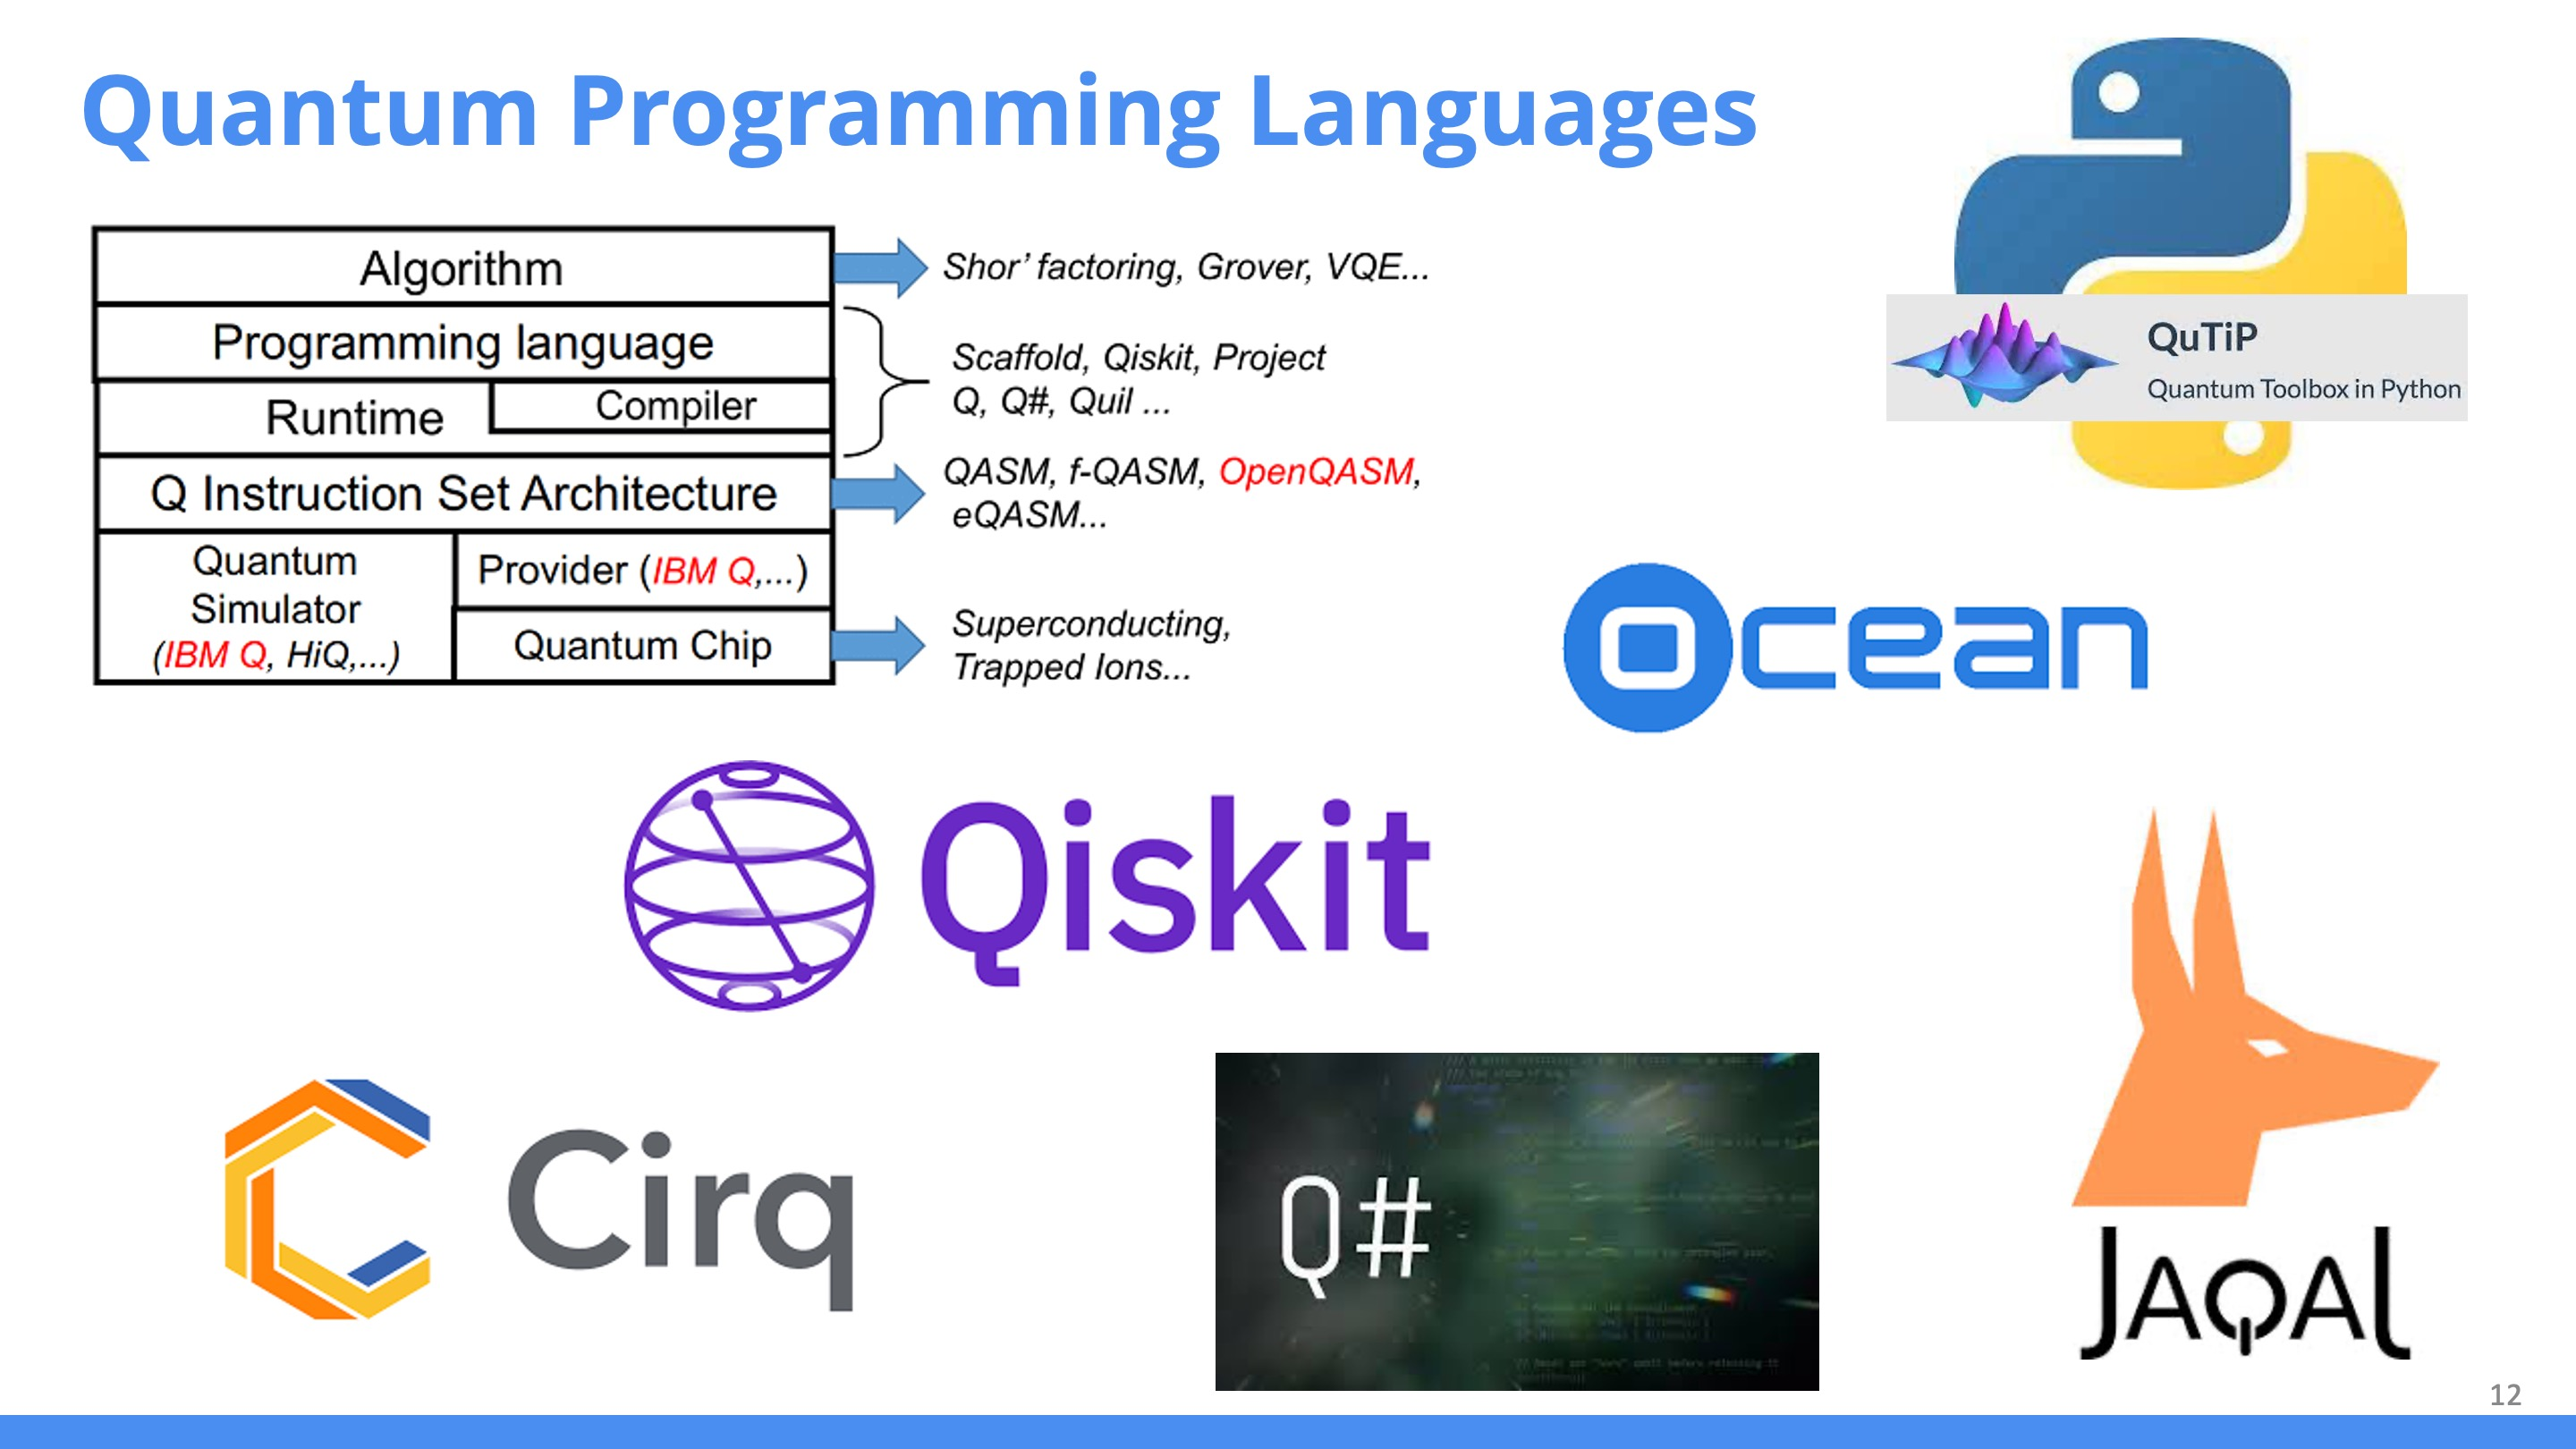
\includegraphics[width=12cm]{fig/Slide12.jpeg}
\end{center}
\end{frame}

\begin{frame}\frametitle{Introduction}
\begin{center}
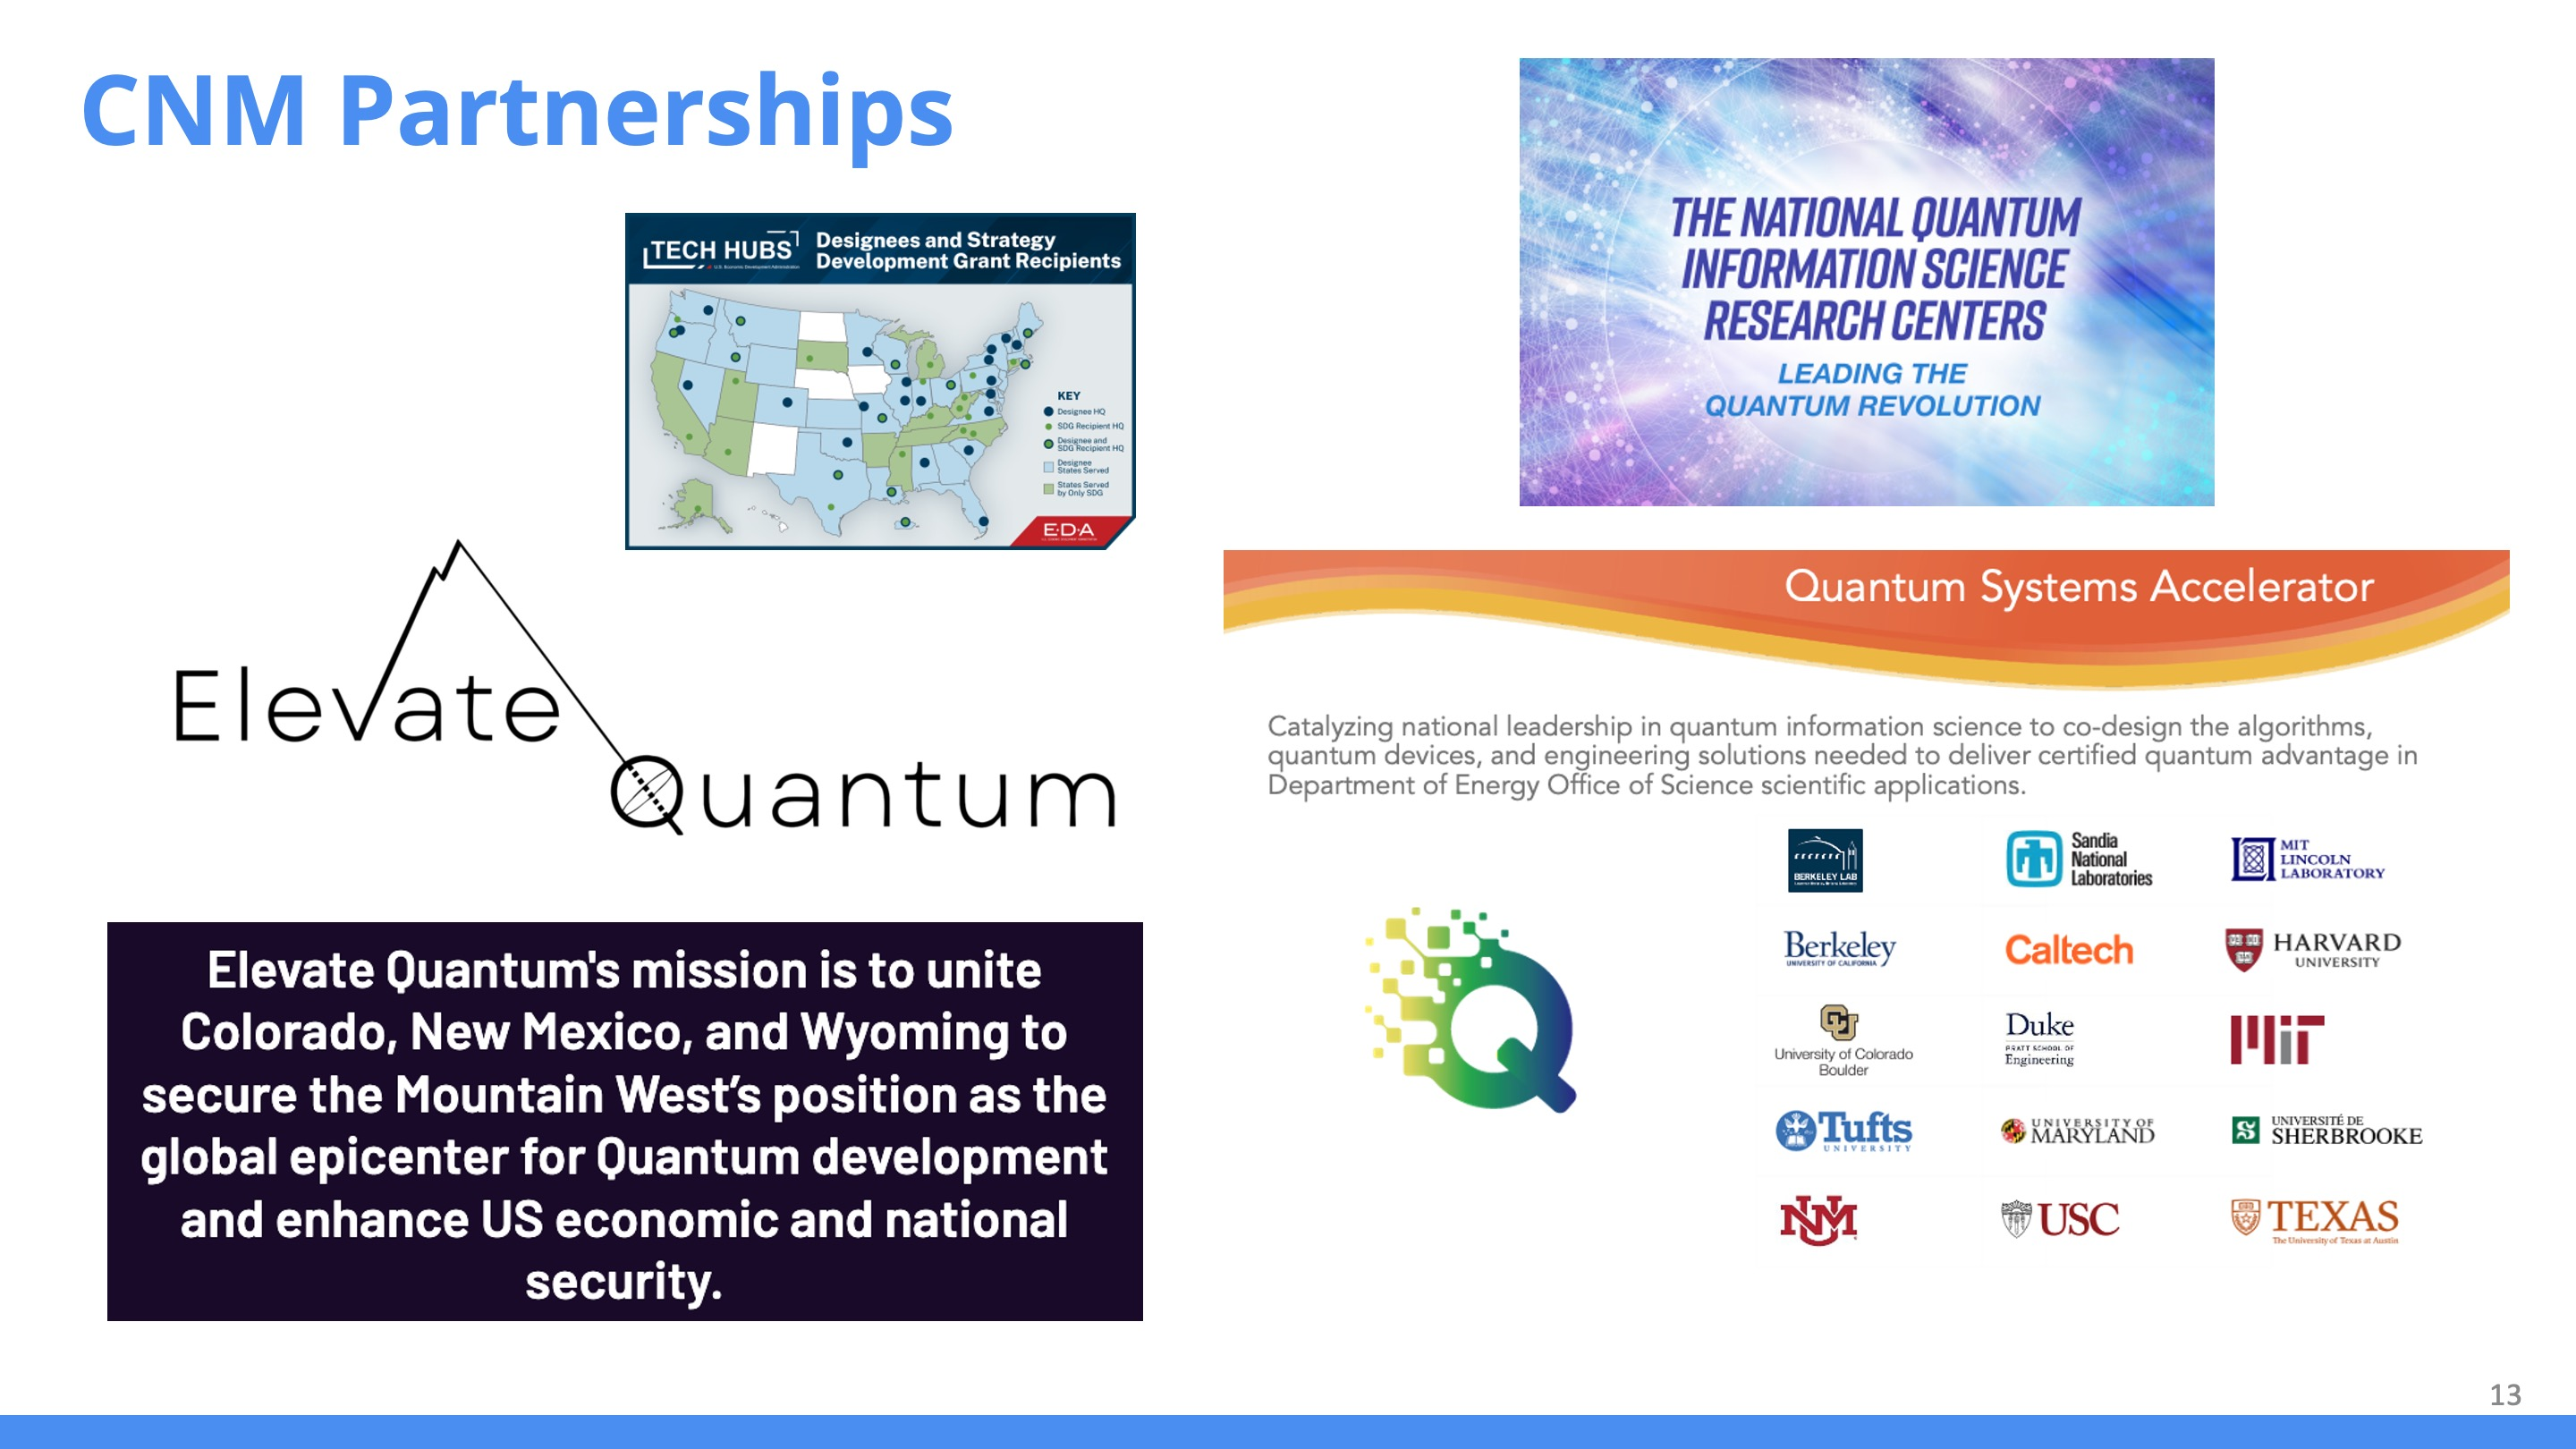
\includegraphics[width=12cm]{fig/Slide13.jpeg}
\end{center}
\end{frame}

\begin{frame}\frametitle{Introduction}
\begin{center}
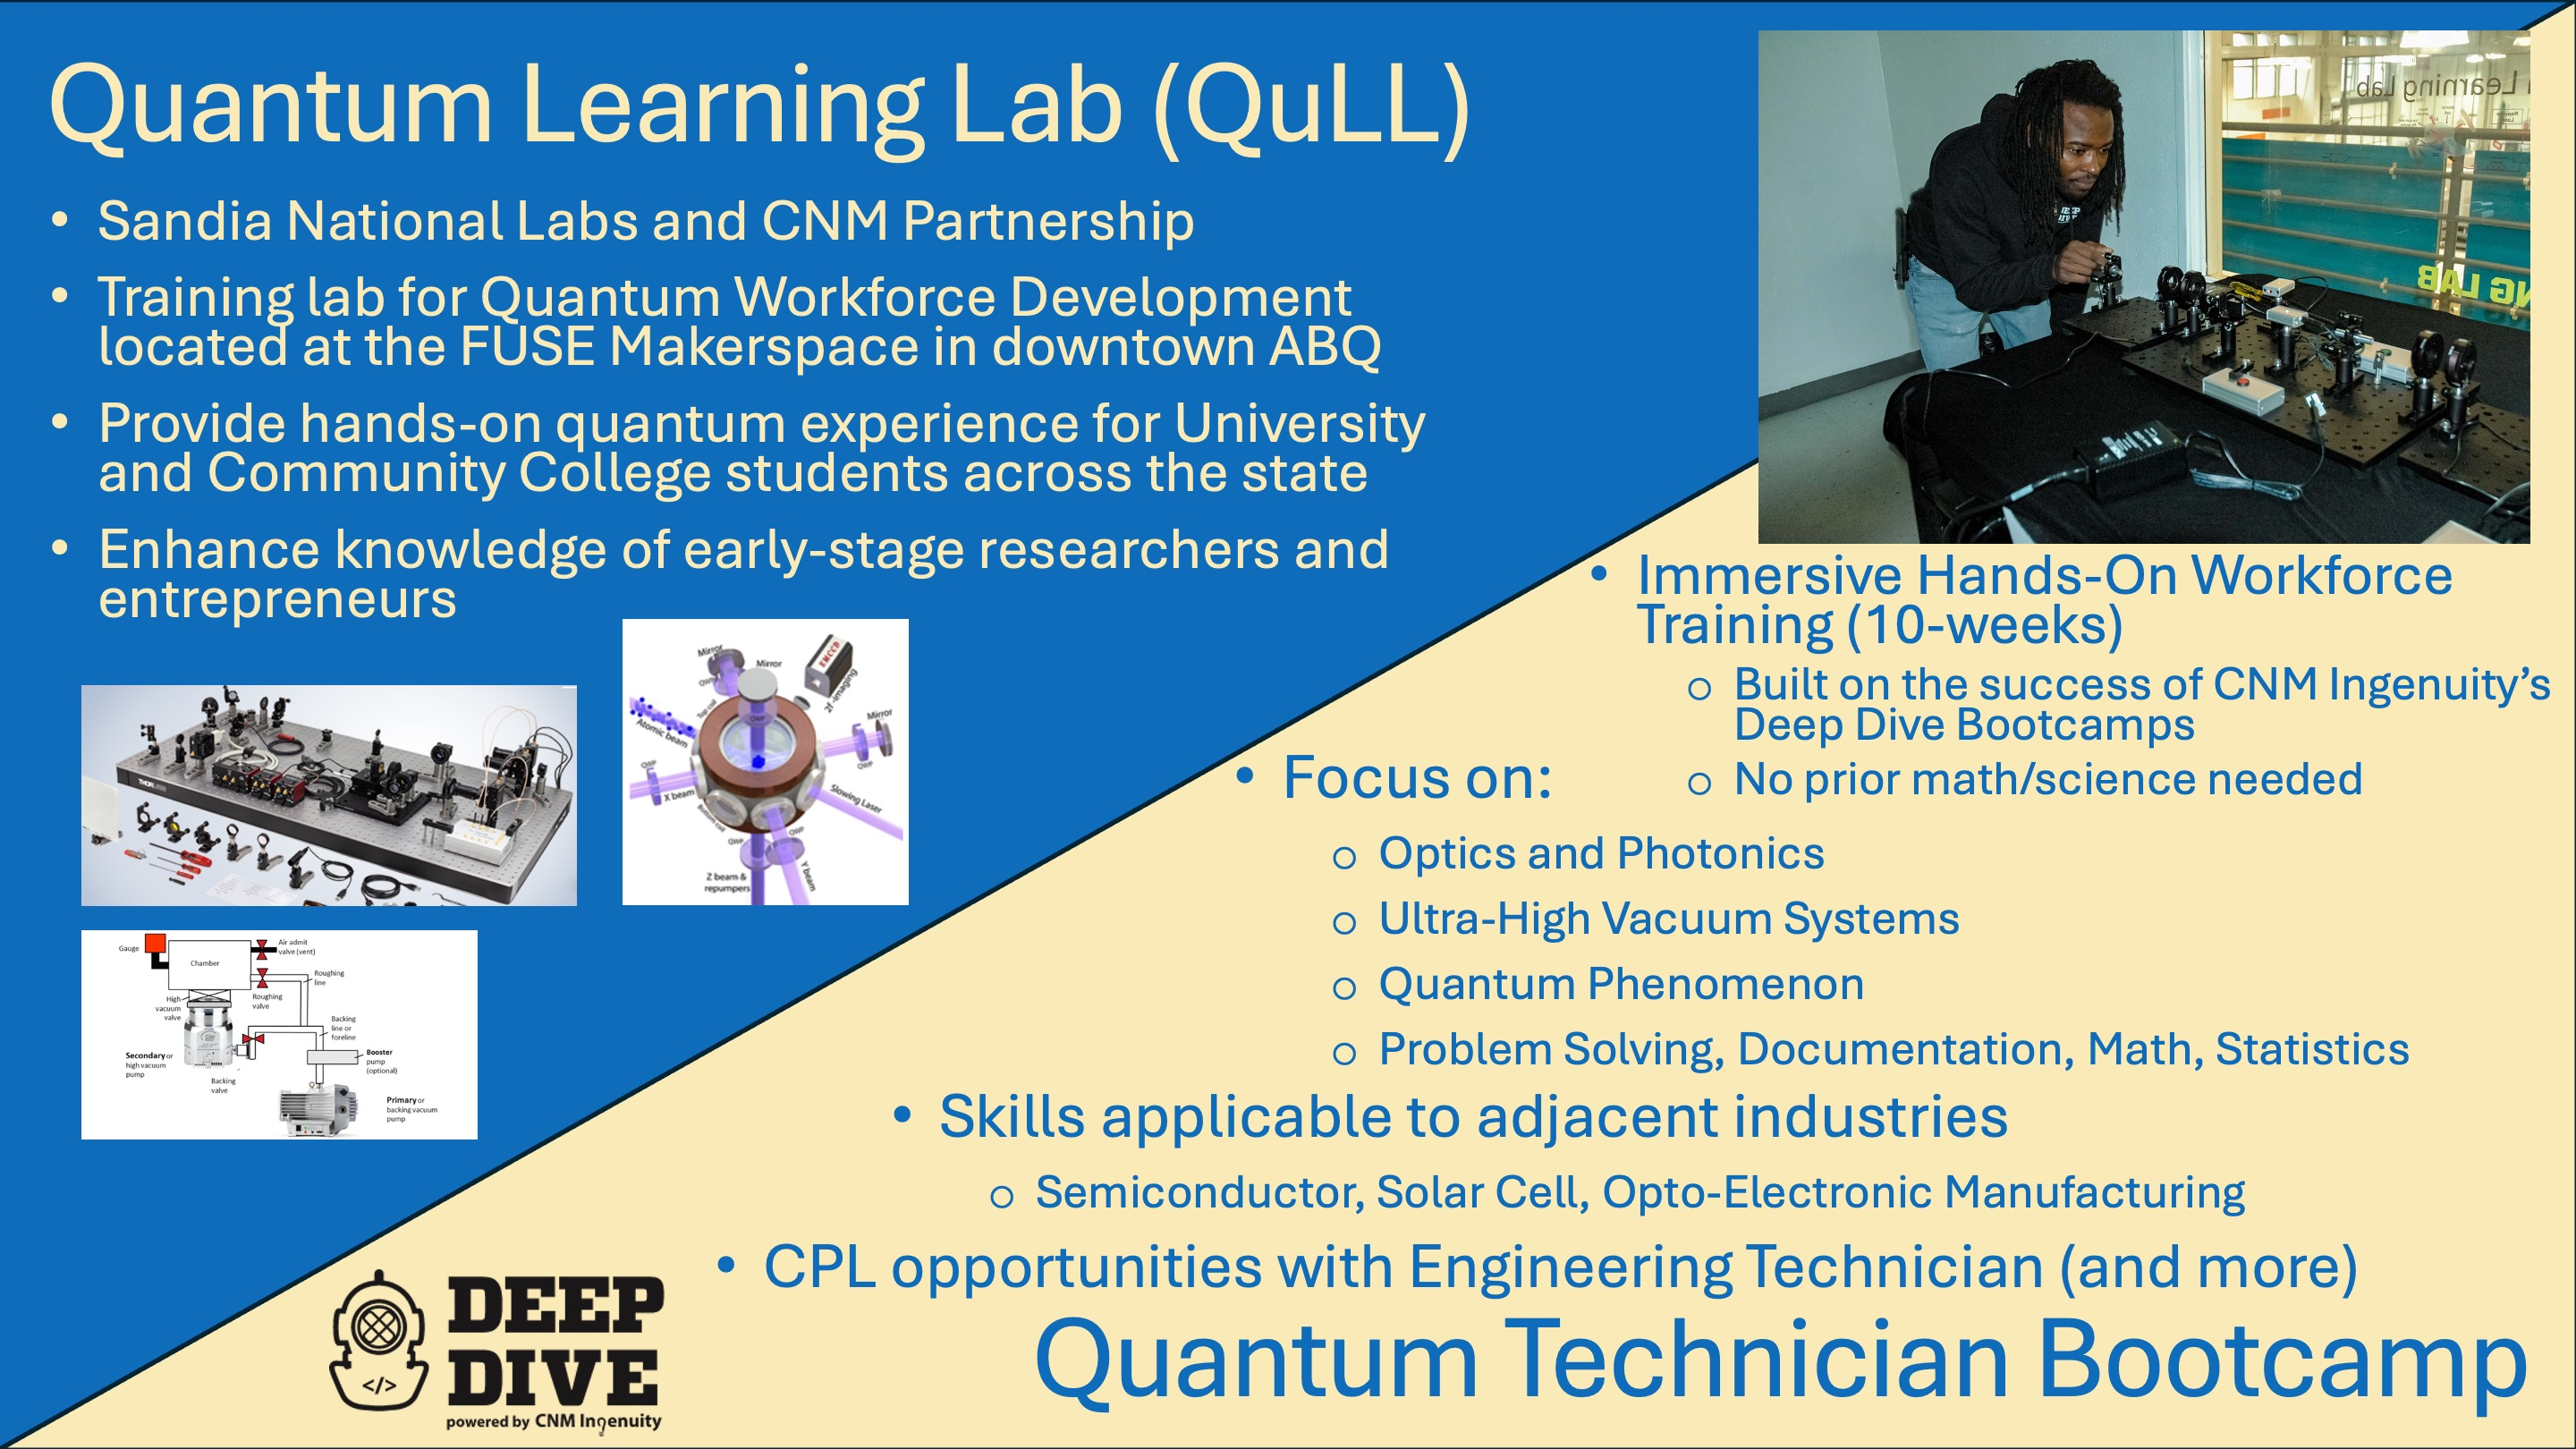
\includegraphics[width=12cm]{fig/Slide14.jpeg}
\end{center}
\end{frame}

\begin{frame}\frametitle{Introduction}
\begin{center}
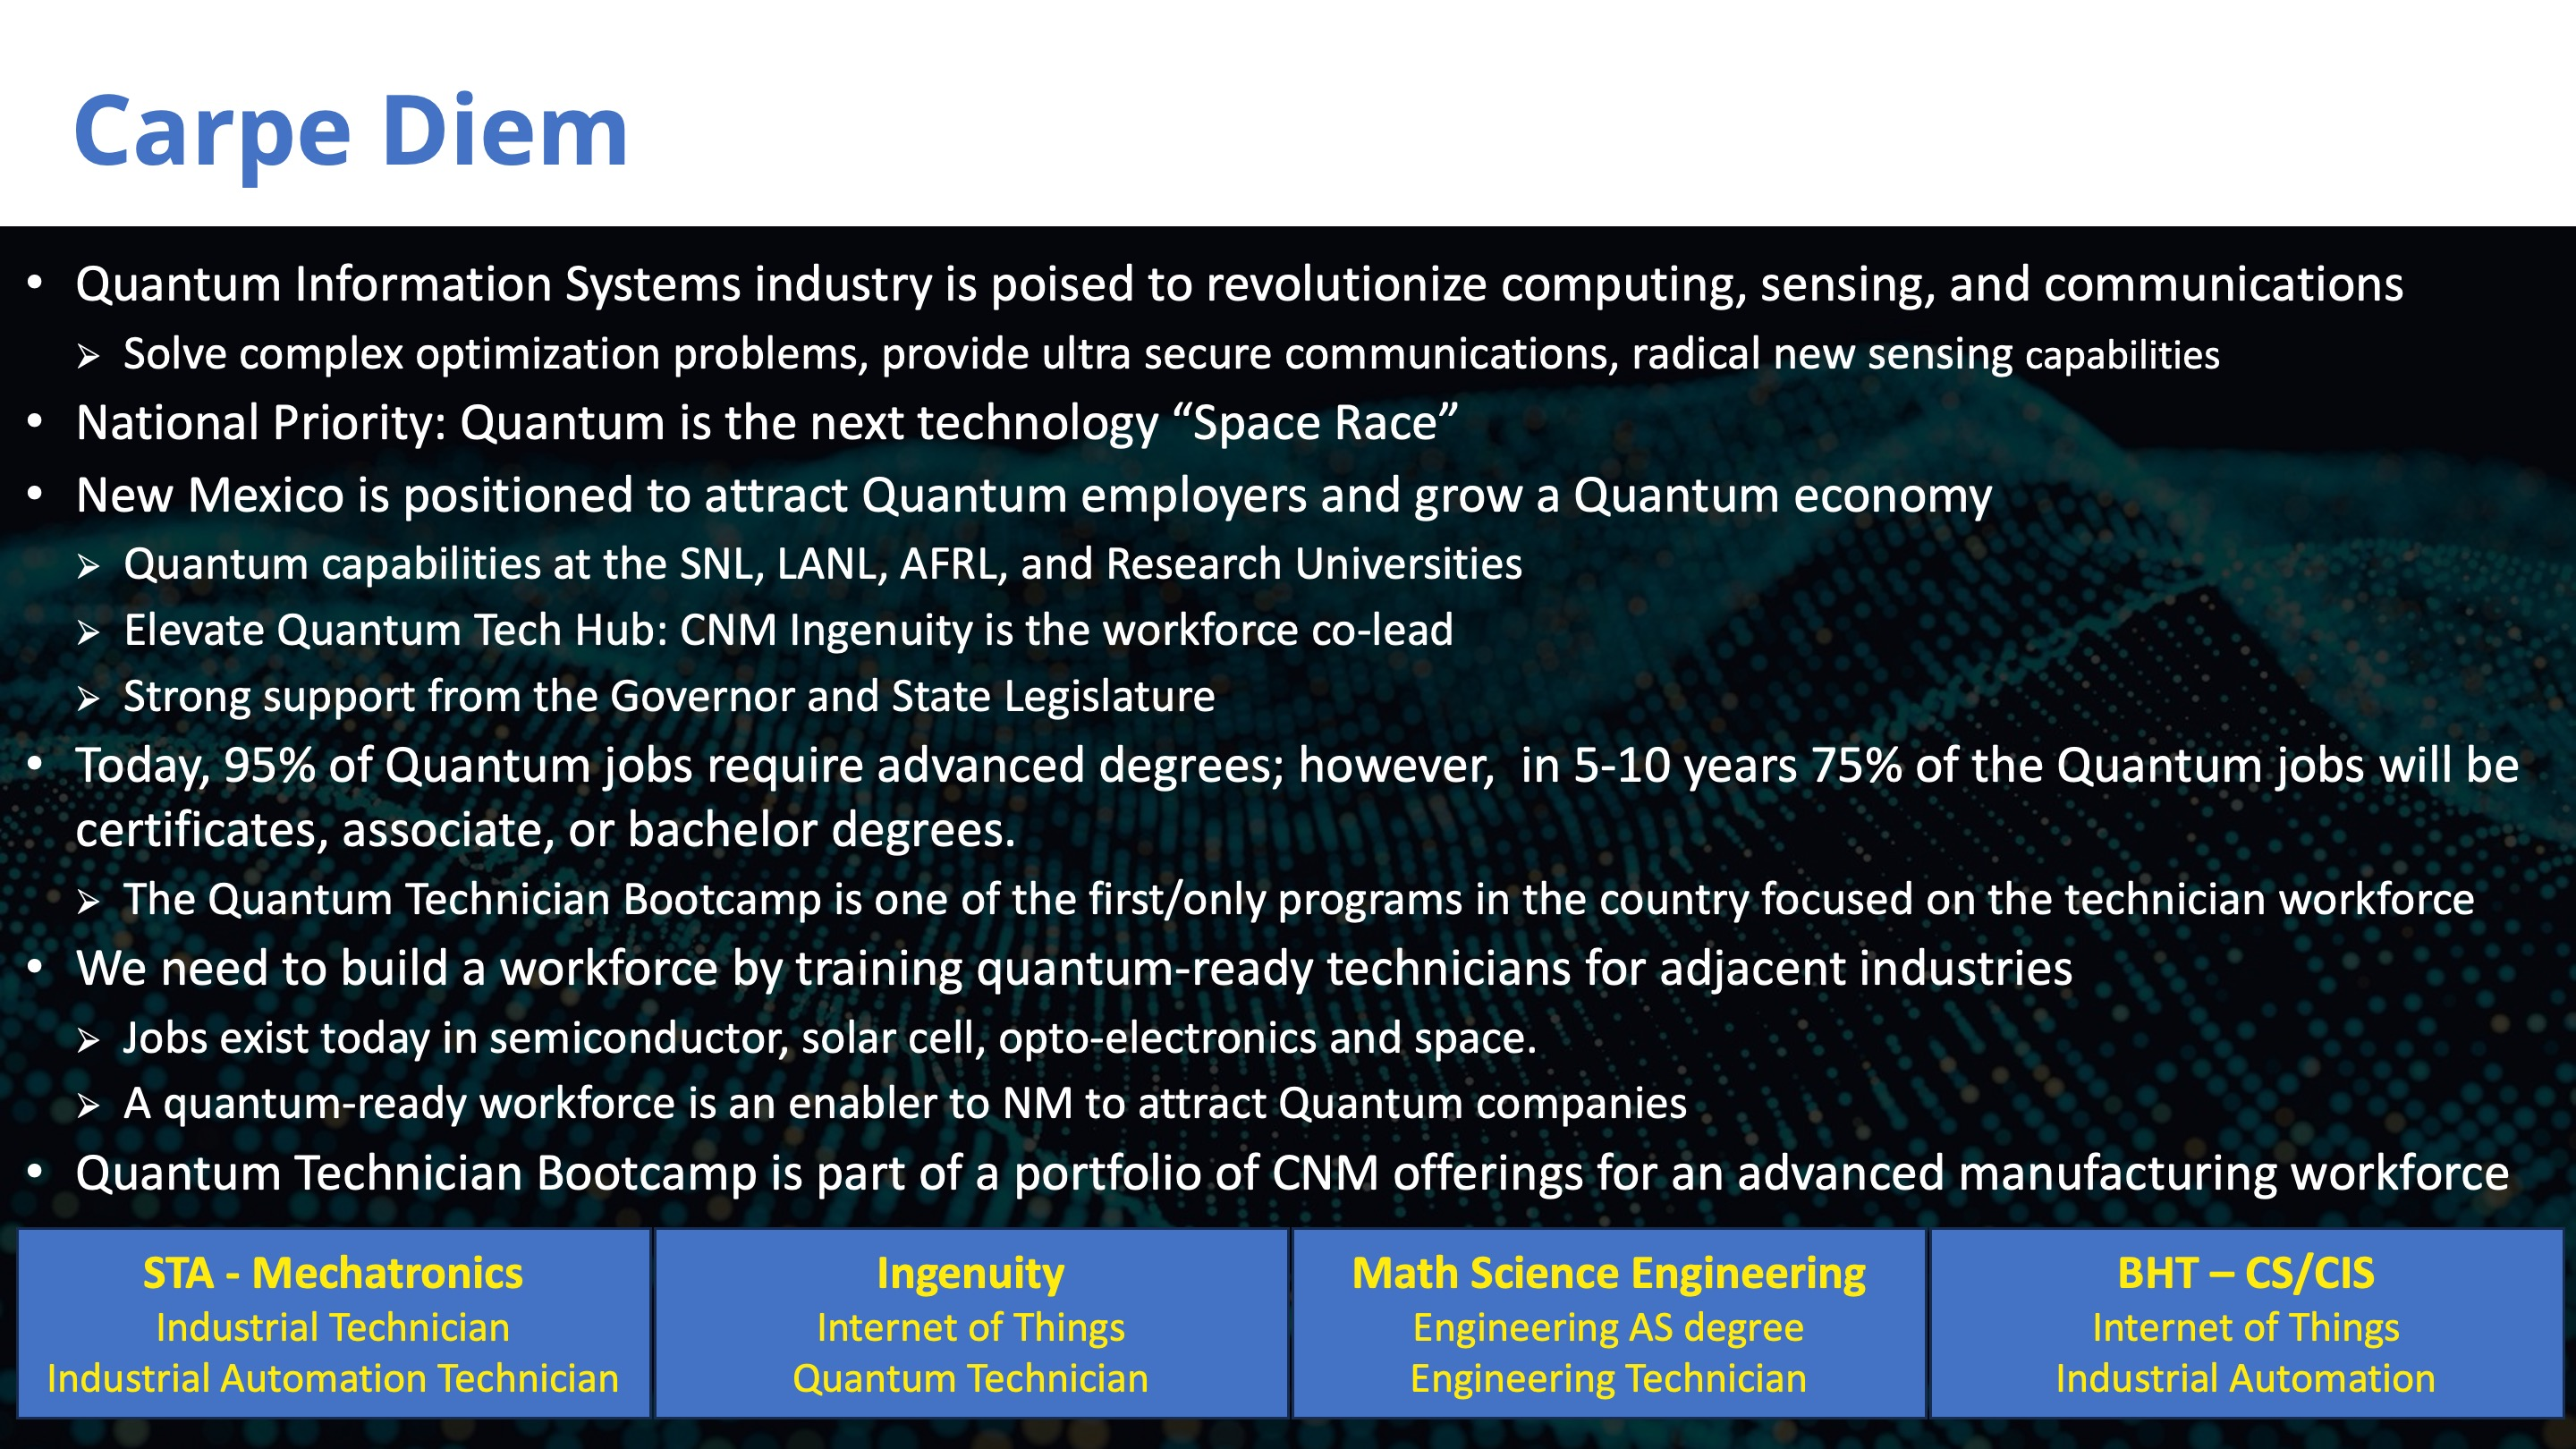
\includegraphics[width=12cm]{fig/Slide15.jpeg}
\end{center}
\end{frame}



\begin{frame}\frametitle{What you will learn}
\begin{itemize}
\item Optics
\item Lasers / Photonics
\item Ultra-High Vacuum Systems
\item Quantum Phenomenon
\item Applied Mathematics
\item Structured Problem Solving
\end{itemize}
\end{frame}


\begin{frame}\frametitle{Brightspace}
\begin{center}
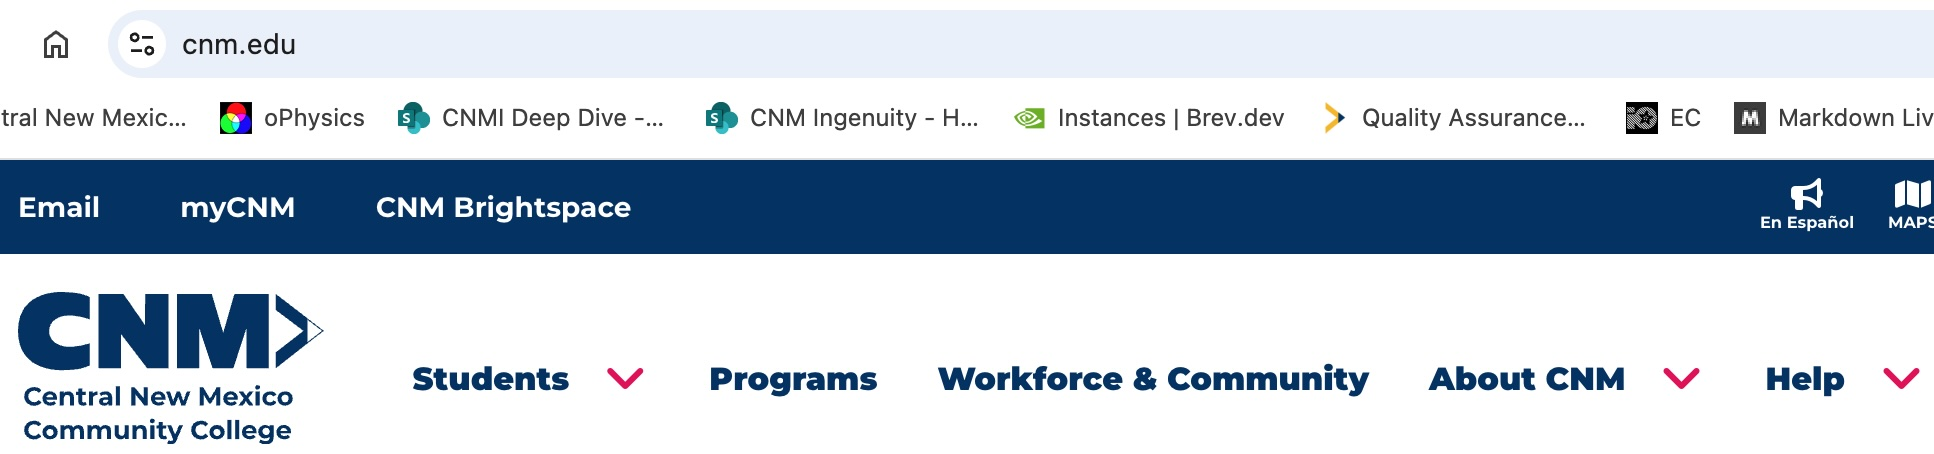
\includegraphics[width=10cm]{fig/brightspace1.jpg}

\vspace{1cm}

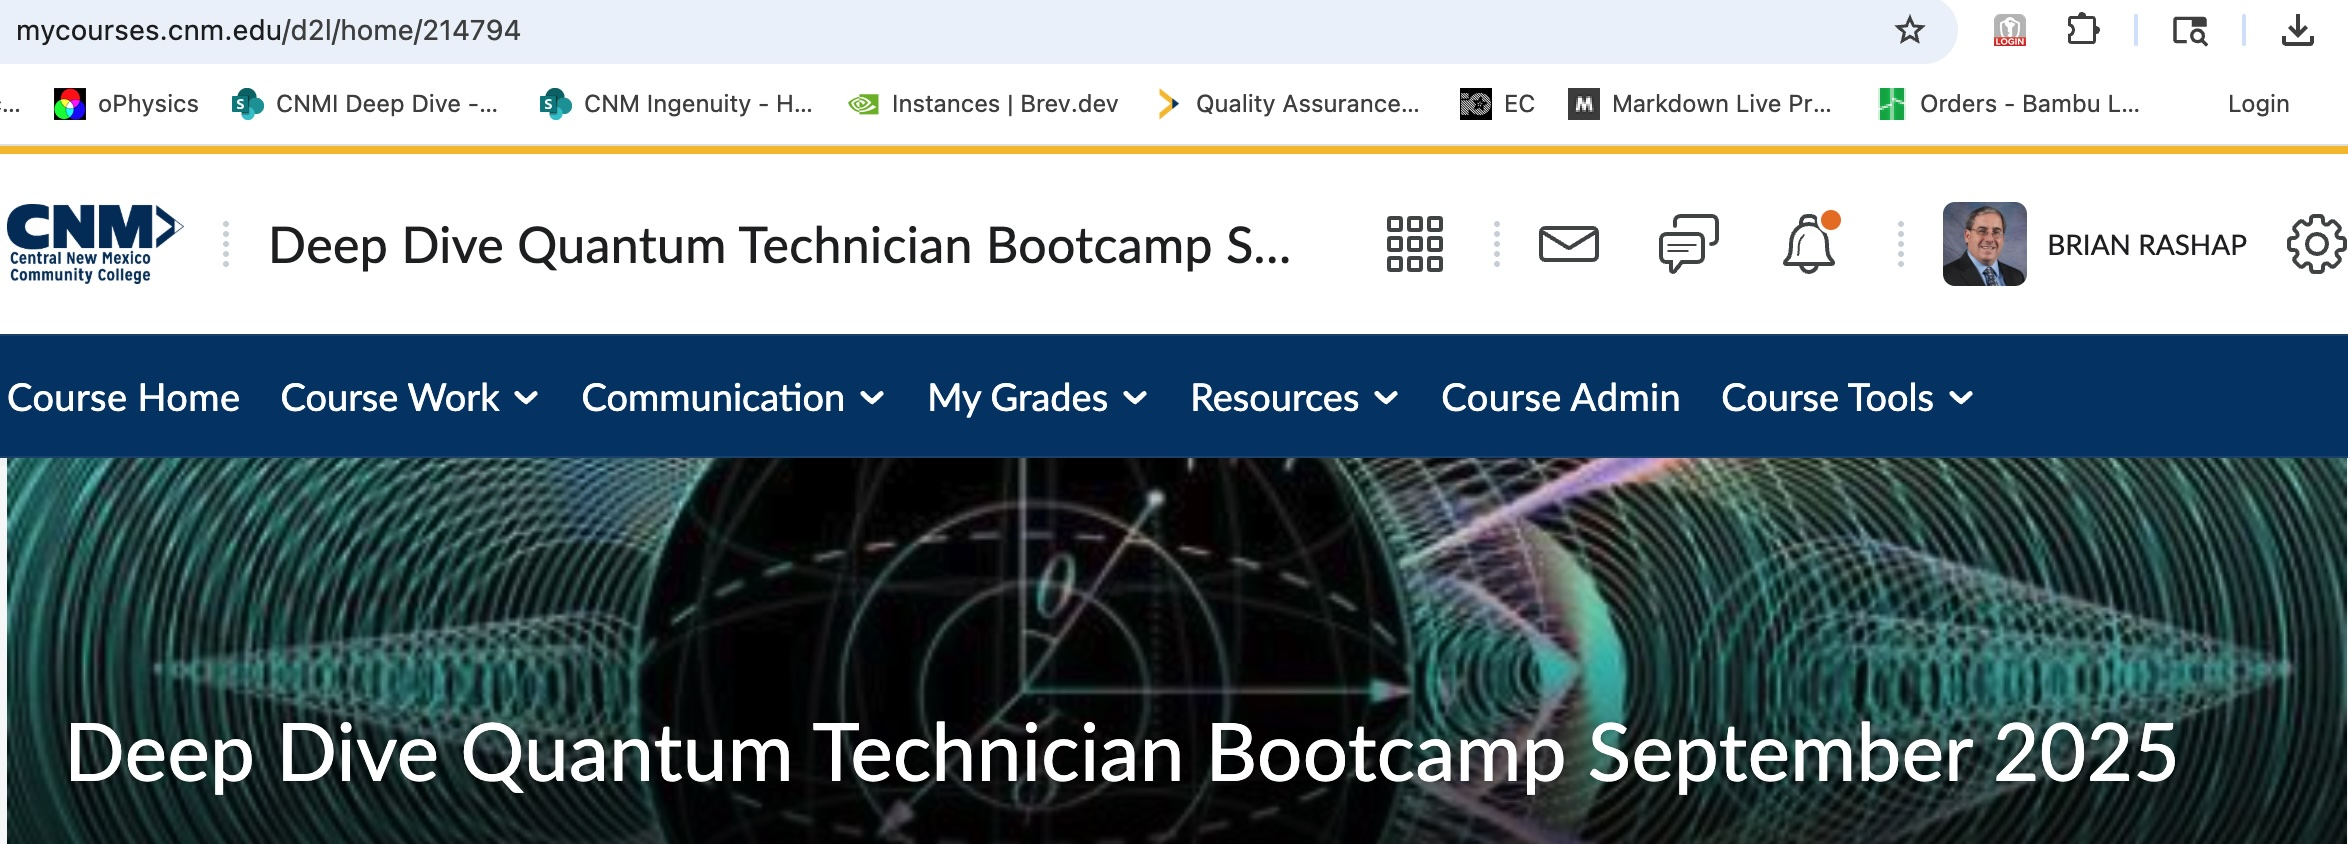
\includegraphics[width=10cm]{fig/brightspace2.jpg}
\end{center}
\end{frame}


\begin{frame}\frametitle{Solidworks - Windows Users}


To install Solidworks (Windows only), go to \url{http://www.SolidWorks.com/SEK}
\begin{itemize}
\item Enter your contact information.
\item Check the radio button “Yes” under "I already have a Serial Number that starts with 9020".
\item Select the version: 2024 SP5.0 and click Request Download.
\item On the next page, Accept the agreement and continue.
\item On the final page, click the Download button to download the SolidWorks Installation Manager.
\item Unzip the files to launch the Installation.
\item Select the option for Individual/On this machine.
\item Install using the following serial number provided by your instructor.
\end{itemize}



\end{frame}

\begin{comment}

macOS and Linux users will use onShape: \url{https://www.onshape.com/en/education/}

2021-2022: 9020005002143476M2TGM8G4
2022-2023: 9020005328617363VNZVR37D


1.  Uninstall any/all previous version of SOLIDWORKS
2.  Go to www.solidworks.com/SEK
3.  Use SEK-ID = XSEK12 and enter all relevant information into the form
4.  Choose 2023 for the most recent version of SOLIDWORKS
5.  You will then be asked to enter the school’s unique SEK Serial Number:
Your Student Download Serial Number is:

9020005723476091HT7RDP86 - (Qty: 60)
9020005723816337C39Z2D27 - (Qty: 20)

* Follow all remaining instructions and accept all defaults
* Your VAR Name is GoEngineer

\end{comment}

\begin{frame}\frametitle{Other Software}
\begin{enumerate}
\item Bambu Studio
	\begin{itemize}
	\item \url{https://bambulab.com/en/download/studio}
	\end{itemize}
\item Microsoft Excel
	\begin{itemize}
	\item \url{https://office365.com}
	\item Log in with your CNM credentials
	\item Download excel (and any other office programs) 
	\end{itemize}
\item Adobe Illustrator 
	\begin{itemize}
	\item \url{https://adobe.com/creativecloud}
	\item Log in with your CNM credentials
	\item Select Work/School account 
	\end{itemize}
\item Octave
	\begin{itemize}
	\item \url{https://octave.org/download}
	\end{itemize}
\item Bookmark the following: 
	\begin{itemize}
	\item \url{https://www.desmos.com}
	\item \url{https://quantum.cloud.ibm.com/composer}
	\item \url{https://colab.research.google.com}
	\end{itemize}
\end{enumerate}
\end{frame}

\begin{frame}\frametitle{Inaugural Cohort}
\begin{center}

\includegraphics[width=10cm]{fig/underconstruction.jpg}
\end{center}
\end{frame}

\begin{frame}\frametitle{Pre Knowledge Check}
\begin{center}

\includegraphics[width=8cm]{fig/precat.jpg}
\end{center}

\vspace{0.25cm}
\begin{itemize}
\item We are assuming no prior knowledge
\item Pre and Post check will be used to help instructional team for future cohorts
\item D) I am not familiar with this concept is an option on every question
\end{itemize}


\end{frame}




\end{document}
